\section{Clasificación de grupos abelianos finitos}

\begin{ejercicio}\label{ej:7.1}
    Calcular los órdenes de todos los elementos de los distintos grupos abelianos de orden $8$, $12$, $16$ y $24$.
    \begin{enumerate}
        \item Sea $G$ un grupo abeliano de $|G| = 8$.
        
        Como $|G|=8=2^3$, por la estructura de los grupos abelianos finitos, tenemos que hay tres posibilidades:
        \begin{enumerate}
            \item $G \cong C_8$.
            
            Como el orden se mantiene bajo isomorfismos, basta con encontrar el orden de los elementos del grupo cíclico $C_8\cong \bb{Z}_8$.
            \begin{equation*}
                O(x) = \frac{8}{\mcd(x, 8)}.
            \end{equation*}

            Por tanto, los órdenes de los elementos de $C_8$ son:
            \begin{equation*}
                O(0) = 1, \quad
                O(1) = O(3) = O(5) = O(7) = 8, \quad
                O(2) = O(6) = 4, \quad
                O(4) = 2.
            \end{equation*}

            Por tanto, hay un elemento de orden $1$, cuatro de orden $8$, dos de orden $4$ y uno de orden $2$.

            \item $G \cong C_4 \oplus C_2$.
            \begin{equation*}
                O(x, y) = \mcm(O(x), O(y))\qquad \forall x \in C_4, y \in C_2.
            \end{equation*}

            Los órdenes de $\bb{Z}_2$ son:
            \begin{equation*}
                O(0) = 1, \quad O(1) = 2.
            \end{equation*}

            Los órdenes de $\bb{Z}_4$ son:
            \begin{equation*}
                O(0) = 1, \quad O(1) = O(3) = 4, \quad O(2) = 2.
            \end{equation*}

            Por tanto, los órdenes de los elementos de $C_4 \oplus C_2$ son:
            \begin{gather*}
                O(0, 0) = 1, \quad
                O(1, 0) = O(1,1) = O(3, 0) = O(3, 1) = 4, \\
                O(2, 0) = O(2, 1) = 2, \quad
                O(0, 1) = 2.
            \end{gather*}
            Por tanto, hay un elemento de orden $1$, cuatro de orden $4$ y tres de orden~$2$.
            \item $G \cong C_2 \oplus C_2 \oplus C_2$.
            
            Los órdenes de $\bb{Z}_2$ son:
            \begin{equation*}
                O(0) = 1, \quad O(1) = 2.
            \end{equation*}
            Por tanto, los órdenes de los elementos de $C_2 \oplus C_2 \oplus C_2$ son:
            \begin{align*}
                O(0, 0, 0) &= 1, \\
                O(x,y,z) &= 2 \qquad \forall x,y,z \in \{0,1\} \text{ tal que } x+y+z \neq 0.
            \end{align*}
            Por tanto, hay un elemento de orden $1$ y siete de orden $2$.
        \end{enumerate}



        \item Sea $G$ un grupo abeliano de $|G| = 12$.
        
        Como $|G|=12=2^2 \cdot 3$, por la estructura de los grupos abelianos finitos, tenemos que hay varias posibilidades:
        \begin{enumerate}
            \item $G \cong C_{12}$.
            
            Como el orden se mantiene bajo isomorfismos, basta con encontrar el orden de los elementos del grupo cíclico $C_{12}\cong \bb{Z}_{12}$.
            \begin{equation*}
                O(x) = \frac{12}{\mcd(x, 12)}.
            \end{equation*}

            Por tanto, los órdenes de los elementos de $C_{12}$ son:
            \begin{gather*}
                O(0) = 1, \quad
                O(1) = O(5) = O(7) = O(11) = 12, \quad
                O(2) = O(10) = 6,\\
                O(3) = O(9) = 4, \quad
                O(4) = O(8) = 3, \quad
                O(6) = 2.
            \end{gather*}

            
            \item $G \cong C_6 \oplus C_2$.
            
            Como el orden se mantiene bajo isomorfismos, basta con encontrar el orden de los elementos del grupo cíclico $C_6\cong \bb{Z}_6$ y de $C_2\cong \bb{Z}_2$.
            Los órdenes de $\bb{Z}_2$ son:
            \begin{equation*}
                O(0) = 1, \quad O(1) = 2.
            \end{equation*}
            Los órdenes de $\bb{Z}_6$ son:
            \begin{equation*}
                O(0) = 1, \quad O(1) = O(5) = 6, \quad O(2) = O(4) = 3, \quad O(3) = 2.
            \end{equation*}

            Por tanto, los órdenes de los elementos de $C_6 \oplus C_2$ son:
            \begin{gather*}
                O(0, 0) = 1, \\
                O(1, 0) = O(5, 0) = O(1, 1) = O(5, 1) = 6, \\
                O(2, 0) = O(4, 0) = 3, \\
                O(2, 1) = O(4, 1) = 6, \\
                O(3, 0) = O(3, 1) = 2, \\
                O(0, 1) = 2.
            \end{gather*}
            
        \end{enumerate}


        \item Sea $G$ un grupo abeliano de $|G| = 16$.
        
        Como $|G|=16=2^4$, por la estructura de los grupos abelianos finitos, tenemos que hay varias posibilidades:
        \begin{enumerate}
            \item $G \cong C_{16}$.
            
            Como el orden se mantiene bajo isomorfismos, basta con encontrar el orden de los elementos del grupo cíclico $C_{16}\cong \bb{Z}_{16}$.
            \begin{equation*}
                O(x) = \frac{16}{\mcd(x, 16)}.
            \end{equation*}
            Por tanto, los órdenes de los elementos de $C_{16}$ son:
            \begin{gather*}
                O(0) = 1, \\
                O(1) = O(3) = O(5) = O(7) = O(9) = O(11) = O(13) = O(15) = 16, \\
                O(2) = O(6) = O(10) = O(14) = 8, \\
                O(4) = O(12) = 4.
            \end{gather*}
            
            \item $G \cong C_8 \oplus C_2$.
            
            Como el orden se mantiene bajo isomorfismos, basta con encontrar el orden de los elementos del grupo cíclico $C_8\cong \bb{Z}_8$ y de $C_2\cong \bb{Z}_2$.
            Los órdenes de $\bb{Z}_2$ son:
            \begin{equation*}
                O(0) = 1, \quad O(1) = 2.
            \end{equation*}

            Los órdenes de $\bb{Z}_8$ los hemos calculado en el primer apartado:
            \begin{equation*}
                O(0) = 1, \quad
                O(1) = O(3) = O(5) = O(7) = 8, \quad
                O(2) = O(6) = 4, \quad
                O(4) = 2.
            \end{equation*}

            Por tanto, los órdenes de los elementos de $C_8 \oplus C_2$ son:
            \begin{gather*}
                O(0, 0) = 1, \qquad O(0,1)= 2, \\
                O(1, 0) = O(3, 0) = O(5, 0) = O(7, 0) = 8, \\
                O(1, 1) = O(3, 1) = O(5, 1) = O(7, 1) = 8, \\
                O(2, 0) = O(6, 0) = O(2, 1) = O(6, 1) = 4, \\
                O(4, 0) = O(4, 1) = 2.
            \end{gather*}

            \item $G \cong C_4 \oplus C_4$.
            
            Como el orden se mantiene bajo isomorfismos, basta con encontrar el orden de los elementos del grupo cíclico $C_4\cong \bb{Z}_4$.
            Los órdenes de $\bb{Z}_4$ son:
            \begin{equation*}
                O(0) = 1, \quad O(1) = O(3) = 4, \quad O(2) = 2.
            \end{equation*}
            Por tanto, los órdenes de los elementos de $C_4 \oplus C_4$ son:
            \begin{gather*}
                O(0, 0) = 1\\
                O(0,1) = O(0,3) = O(1,1) = O(1,3) = O(2,1) = O(2,3) = O(3,1) = O(3,3) = 4, \\
                O(1,0) = O(1,2) = O(3,0) = O(3,2) = 4, \\
                O(0,2) = O(2,0) = O(2,2) = 2
            \end{gather*}
            \item $G \cong C_4 \oplus C_2 \oplus C_2$.
            
            Como el orden se mantiene bajo isomorfismos, basta con encontrar el orden de los elementos del grupo $C_4\oplus C_2 \oplus C_2$. Los órdenes de $C_4\oplus C_2$ ya los hemos calculado anteriormente:
            \begin{gather*}
                O(0, 0) = 1, \\
                O(1, 0) = O(1,1) = O(3, 0) = O(3, 1) = 4, \\
                O(2, 0) = O(2, 1) = 2, \\
                O(0, 1) = 2.
            \end{gather*}

            Los órdenes de $C_2$ son:
            \begin{equation*}
                O(0) = 1, \quad O(1) = 2.
            \end{equation*}

            Por tanto, los órdenes de los elementos de $C_4 \oplus C_2 \oplus C_2$ son:
            \begin{gather*}
                O(0, 0, 0) = 1, \\
                O(1, 0, 0) = O(1, 1, 0) = O(3, 0, 0) = O(3, 1, 0) = 4, \\
                O(2, 0, 0) = O(2, 1, 0) = 2, \\
                O(0, 1, 0) = 2, \\
                O(0, 0, 1) = 2, \\
                O(1, 0, 1) = O(1, 1, 1) = O(3, 0, 1) = O(3, 1, 1) = 4, \\
                O(2, 0, 1) = O(2, 1, 1) = 2, \\
                O(0, 1, 1) = 2.
            \end{gather*}
            
            \item $G \cong C_2 \oplus C_2 \oplus C_2 \oplus C_2$.
            
            Como el orden se mantiene bajo isomorfismos, basta con encontrar el orden de los elementos del grupo $C_2\oplus C_2 \oplus C_2 \oplus C_2$. Los órdenes de $C_2\oplus C_2 \oplus C_2$ ya los hemos calculado anteriormente:
            \begin{align*}
                O(0, 0, 0) &= 1, \\
                O(x, y, z) &= 2 \qquad \forall x,y,z \in \{0,1\} \text{ tal que } x+y+z \neq 0.
            \end{align*}

            Por tanto, los órdenes de los elementos de $C_2 \oplus C_2 \oplus C_2 \oplus C_2$ son:
            \begin{align*}
                O(0, 0, 0, 0) &= 1, \\
                O(x, y, z, w) &= 2 \qquad \forall x,y,z,w \in \{0,1\} \text{ tal que } x+y+z+w \neq 0.
            \end{align*}
        \end{enumerate}

        \item Sea $G$ un grupo abeliano de $|G| = 24$.
        
        Como $|G|=24=2^3 \cdot 3$, por la estructura de los grupos abelianos finitos, tenemos que hay varias posibilidades:
        \begin{enumerate}
            \item $G \cong C_{24}$.
            
            Como el orden se mantiene bajo isomorfismos, basta con encontrar el orden de los elementos del grupo cíclico $C_{24}\cong \bb{Z}_{24}$.
            \begin{equation*}
                O(x) = \frac{24}{\mcd(x, 24)}.
            \end{equation*}

            Por tanto, los órdenes de los elementos de $C_{24}$ son:
            \begin{gather*}
                O(0) = 1, \\
                O(1) = O(5) = O(7) = O(11) = O(13) = O(17) = O(19) = O(23) = 24, \\
                O(2) = O(10) = O(14) = O(22) = 12, \\
                O(3) = O(9) = O(15) = 8, \\
                O(4) = O(20) = 6, \\
                O(6) = O(18) = 4, \\
                O(8) = O(16) = 3, \\
                O(12) = 2.
            \end{gather*}
            
            \item $G \cong C_{12} \oplus C_2$.
            
            Como el orden se mantiene bajo isomorfismos, basta con encontrar el orden de los elementos del grupo cíclico $C_{12}\cong \bb{Z}_{12}$ y de $C_2\cong \bb{Z}_2$.
            Los órdenes de $\bb{Z}_12$ los hemos calculado anteriormente:
            \begin{gather*}
                O(0) = 1, \\
                O(1) = O(5) = O(7) = O(11) = 12, \\
                O(2) = O(10) = 6, \\
                O(3) = O(9) = 4, \\
                O(4) = O(8) = 3, \\
                O(6) = 2.
            \end{gather*}

            Los órdenes de $\bb{Z}_2$ son:
            \begin{equation*}
                O(0) = 1, \quad O(1) = 2.
            \end{equation*}

            Por tanto, los órdenes de los elementos de $C_{12} \oplus C_2$ son:
            \begin{gather*}
                O(0, 0) = 1, \\
                O(1, 0) = O(5, 0) = O(7, 0) = O(11, 0) = 12, \\
                O(2, 0) = O(10, 0) = 6, \\
                O(3, 0) = O(9, 0) = 4, \\
                O(4, 0) = O(8, 0) = 3, \\
                O(6, 0) = 2, \\
                O(0, 1) = 2, \\
                O(1, 1) = O(5, 1) = O(7, 1) = O(11, 1) = 12, \\
                O(2, 1) = O(10, 1) = 6, \\
                O(3, 1) = O(9, 1) = 4, \\
                O(4, 1) = O(8, 1) = 6, \\
                O(6, 1) = 2.
            \end{gather*}
            
            \item $G \cong C_6 \oplus C_2 \oplus C_2$.
            
            Como el orden se mantiene bajo isomorfismos, basta con encontrar el orden de los elementos del grupo $C_6\oplus C_2 \oplus C_2$. Los órdenes de $C_6\oplus C_2$ ya los hemos calculado anteriormente:
            \begin{gather*}
                O(0, 0) = 1, \\
                O(1, 0) = O(5, 0) = O(1, 1) = O(5, 1) = 6, \\
                O(2, 0) = O(4, 0) = 3, \\
                O(2, 1) = O(4, 1) = 6, \\
                O(3, 0) = O(3, 1) = 2, \\
                O(0, 1) = 2.
            \end{gather*}

            Los órdenes de $C_2$ son:
            \begin{equation*}
                O(0) = 1, \quad O(1) = 2.
            \end{equation*}

            Por tanto, los órdenes de los elementos de $C_6 \oplus C_2 \oplus C_2$ son:
            \begin{gather*}
                O(0, 0, 0) = 1, \\
                O(1, 0, 0) = O(5, 0, 0) = O(1, 1, 0) = O(5, 1, 0) = 6, \\
                O(2, 0, 0) = O(4, 0, 0) = 3, \\
                O(2, 1, 0) = O(4, 1, 0) = 6, \\
                O(3, 0, 0) = O(3, 1, 0) = 2, \\
                O(0, 1, 0) = 2, \\
                O(0, 0, 1) = 2, \\
                O(1, 0, 1) = O(5, 0, 1) = O(1, 1, 1) = O(5, 1, 1) = 6, \\
                O(2, 0, 1) = O(4, 0, 1) = O(2, 1, 1) = O(4, 1, 1) = 6, \\
                O(3, 0, 1) = O(3, 1, 1) = 2, \\
                O(0, 1, 1) = 2.
            \end{gather*}
        \end{enumerate}







    \end{enumerate}
\end{ejercicio}

\begin{ejercicio}\label{ej:7.2}
    Para los siguientes grupos calcular sus descomposiciones cíclicas.
    \begin{enumerate}
        \item $G_1 = \{1, 8, 12, 14, 18, 21, 27, 31, 34, 38, 44, 47, 51, 53, 57, 64\}$ con operación dada por multiplicación módulo $65$.\\
        
        Vemos que $G_1$ es un abeliano con $|G_1| = 16$. Entonces, por el Ejercicio~\ref{ej:7.1}, sabemos que $G_1$ es isomorfo a uno de los siguientes grupos:
        \begin{enumerate}
            \item $C_{16}$.
            \item $C_8 \oplus C_2$.
            \item $C_4 \oplus C_4$.
            \item $C_4 \oplus C_2 \oplus C_2$.
            \item $C_2 \oplus C_2 \oplus C_2 \oplus C_2$.
        \end{enumerate}

        Para distinguir, calculamos los órdenes de los elementos de $G_1$:
        \begin{gather*}
            O(1) = 1, \\
            O(8) = O(12) = O(18) = O(21) = O(27) = O(31) = O(34) = 4\\
            O(38) = O(44) = O(47) = O(53) = O(57) = 4, \\
            O(14) = O(51) = O(64) = 2.
        \end{gather*}

        Por tanto, la única posibilidad es que $G_1 \cong C_4 \oplus C_4$.
        \item $G_2 = \{1, 8, 17, 19, 26, 28, 37, 44, 46, 53, 62, 64, 71, 73, 82, 89, 91, 98, 107,109, 116, 118, 127, 134\}$ con operación dada por multiplicación módulo $135$.
        
        Vemos que $G_2$ es un abeliano con $|G_2| = 24$. Entonces, por el Ejercicio~\ref{ej:7.1}, sabemos que $G_2$ es isomorfo a uno de los siguientes grupos:
        \begin{enumerate}
            \item $C_{24}$.
            \item $C_{12} \oplus C_2$.
            \item $C_6 \oplus C_2 \oplus C_2$.
        \end{enumerate}

        Para distinguir, calculamos los órdenes de los elementos de $G_2$ (es tedioso, pero sencillo. En nuestro caso, lo hemos implementado mediante un sencillo programa). Nos bastaría con calcular:
        \begin{gather*}
            O(28)=O(53)=O(82)=O(107)=4
        \end{gather*}
        Por tanto, la única posibilidad es que:
        \begin{equation*}
            G_2 \cong C_6 \oplus C_2 \oplus C_2.
        \end{equation*}
        \item $G_3 = \{1, 7, 17, 23, 49, 55, 65, 71\}$ con operación dada por multiplicación módulo $96$.
        
        Vemos que $G_3$ es un abeliano con $|G_3| = 8$. Entonces, por el Ejercicio~\ref{ej:7.1}, sabemos que $G_3$ es isomorfo a uno de los siguientes grupos:
        \begin{enumerate}
            \item $C_8$.
            \item $C_4 \oplus C_2$.
            \item $C_2 \oplus C_2 \oplus C_2$.
        \end{enumerate}

        Para distinguir, calculamos los órdenes de los elementos de $G_3$. De nuevo, es tedioso, pero sencillo. Basta con calcular:
        \begin{equation*}
            O(17) = O(49) = O(65) = 2\qquad O(7)=4
        \end{equation*}

        Por tanto, la única posibilidad es que:
        \begin{equation*}
            G_3 \cong C_4 \oplus C_2.
        \end{equation*}
        \item $G_4 = \{1, 4, 11, 14, 16, 19, 26, 29, 31, 34, 41, 44\}$ con operación dada por multiplicación módulo $45$.
        
        Vemos que $G_4$ es un abeliano con $|G_4| = 12$. Entonces, por el Ejercicio~\ref{ej:7.1}, sabemos que $G_4$ es isomorfo a uno de los siguientes grupos:
        \begin{enumerate}
            \item $C_{12}$.
            \item $C_6 \oplus C_2$.
        \end{enumerate}
        Para distinguir, calculamos los órdenes de los elementos de $G_4$. De nuevo, es tedioso, pero sencillo. Basta con calcular:
        \begin{gather*}
            O(19)=O(26)=O(44)=2
        \end{gather*}

        Por tanto, la única posibilidad es que:
        \begin{equation*}
            G_4 \cong C_6 \oplus C_2.
        \end{equation*}
    \end{enumerate}
\end{ejercicio}

\begin{ejercicio}\label{ej:7.3}
    Calcular la descomposición cíclica y cíclica primaria de los grupos abelianos $C_{24} \oplus C_{40} \oplus C_{35}$ y $C_{14} \oplus C_{100} \oplus C_{40}$. ¿Son isomorfos?\\

    Tenemos que:
    \begin{align*}
        24&=2^3 \cdot 3, \\
        40&=2^3 \cdot 5, \\
        35&=5 \cdot 7, \\
        14&=2 \cdot 7, \\
        100&=2^2 \cdot 5^2, \\
        40&=2^3 \cdot 5.
    \end{align*}

    Por tanto, vemos a simple vista sin necesidad de hacer cálculos que no tienen el mismo orden, luego no son isomorfos.
    Trabajamos ahora con cada uno por separado.
    \begin{enumerate}
        \item Para $C_{24} \oplus C_{40} \oplus C_{35}$:
        
        Tenemos que:
        \begin{align*}
            C_{24} \oplus C_{40} \oplus C_{35} &\cong C_{2^3} \oplus C_3 \oplus C_{2^3} \oplus C_5 \oplus C_{5} \oplus C_7 \\
            &\cong C_{2^3} \oplus C_{2^3} \oplus C_3 \oplus C_5 \oplus C_5 \oplus C_7
        \end{align*}

        Por tanto, esa es la descomposición cíclica primaria:
        \begin{equation*}
            C_{24} \oplus C_{40} \oplus C_{35} \cong C_{2^3} \oplus C_{2^3} \oplus C_3 \oplus C_5 \oplus C_5 \oplus C_7.
        \end{equation*}

        En vistas de calcular la descomposición cíclica, tenemos la siguiente matriz:
        \begin{equation*}
            \begin{pmatrix}
                2^3 & 2^3\\
                3 & 1\\
                5 & 5\\
                7 & 1
            \end{pmatrix}
            \Longrightarrow
            \left\{
                \begin{array}{l}
                    d_1 = 2^3\cdot 3\cdot 5\cdot 7 = 840, \\
                    d_2 = 2^3\cdot 5 = 40
                \end{array}
            \right.
        \end{equation*}

        Por tanto, la descomposición cíclica es:
        \begin{equation*}
            C_{24} \oplus C_{40} \oplus C_{35} \cong C_{840} \oplus C_{40}.
        \end{equation*}

        \item Para $C_{14} \oplus C_{100} \oplus C_{40}$:
        
        Tenemos que:
        \begin{align*}
            C_{14} \oplus C_{100} \oplus C_{40} &\cong C_{2} \oplus C_7 \oplus C_{2^2} \oplus C_{5^2} \oplus C_{2^3} \oplus C_5 \\
            &\cong C_{2^3}\oplus C_{2^2} \oplus C_2 \oplus C_{5^2} \oplus C_5 \oplus C_7
        \end{align*}
        Por tanto, esa es la descomposición cíclica primaria:
        \begin{equation*}
            C_{14} \oplus C_{100} \oplus C_{40} \cong C_{2^3}\oplus C_{2^2} \oplus C_2 \oplus C_{5^2} \oplus C_5 \oplus C_7.
        \end{equation*}
        En vistas de calcular la descomposición cíclica, tenemos la siguiente matriz:
        \begin{equation*}
            \begin{pmatrix}
                2^3 & 2^2 & 2\\
                5^2 & 5 & 1\\
                7 & 1 & 1
            \end{pmatrix}
            \Longrightarrow
            \left\{
                \begin{array}{l}
                    d_1 = 2^3\cdot 5^2\cdot 7 = 1400, \\
                    d_2 = 2^2\cdot 5 = 20, \\
                    d_3 = 2
                \end{array}
            \right.
        \end{equation*}

        Por tanto, la descomposición cíclica es:
        \begin{equation*}
            C_{14} \oplus C_{100} \oplus C_{40} \cong C_{1400} \oplus C_{20} \oplus C_2.
        \end{equation*}
    \end{enumerate}

    Como vemos, las descomposiciones cíclicas son diferentes, lo que también nos indica que los grupos no son isomorfos.
\end{ejercicio}

\begin{ejercicio}\label{ej:7.4}
    Sea $G$ el grupo de las simetrías de un rectángulo (no cuadrado). Probar que $G$ es un grupo abeliano. Calcular sus descomposiciones cíclica y cíclica primaria.\\


    Las simetrías de un rectángulo se muestran en la Figura~\ref{fig:simetria_rectangulo}.
    \begin{figure}[h]
        \centering
        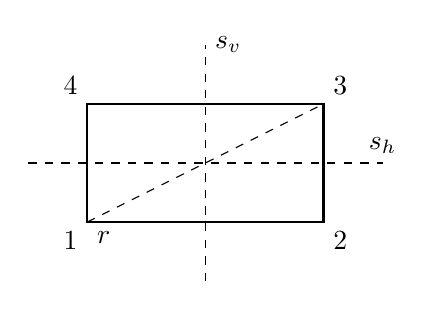
\begin{tikzpicture}[scale=1.5]
            \draw[thick] (0,0) rectangle (2,1);
            
            % Notamos los 4 vértices
            \node at (0,0) [below left] {$1$};
            \node at (2,0) [below right] {$2$};
            \node at (2,1) [above right] {$3$};
            \node at (0,1) [above left] {$4$};

            % Rotación de 180 grados. Diagonal desde 1 a 3
            \draw[dashed] (0,0) -- (2,1) node [pos=0, below right] {$r$};

            % Simetrias eje vertical y horizontal
            \draw[dashed] (1,-0.5) -- (1,1.5) node [pos=1, right] {$s_v$};
            \draw[dashed] (-0.5,0.5) -- (2.5,0.5) node [pos=1, above] {$s_h$};
        \end{tikzpicture}
        \caption{Simetrías de un rectángulo.}
        \label{fig:simetria_rectangulo}
    \end{figure}
    Para ver que se trata de un grupo, damos su tabla de Cayley:
    \begin{equation*}
        \begin{tabular}{c|cccc}
            $\cdot$ & $e$ & $r$ & $s_v$ & $s_h$ \\
            \hline
            $e$ & $e$ & $r$ & $s_v$ & $s_h$ \\
            $r$ & $r$ & $e$ & $s_h$ & $s_v$ \\
            $s_v$ & $s_v$ & $s_h$ & $e$ & $r$ \\
            $s_h$ & $s_h$ & $s_v$ & $r$ & $e$
        \end{tabular}
    \end{equation*}

    Como vemos, $G$ es un grupo. Además, es abeliano porque la tabla es simétrica respecto a la diagonal principal. Como $|G|=4$, hay dos opciones:
    \begin{enumerate}
        \item $G \cong C_4$.
        \item $G \cong C_2 \oplus C_2$.
    \end{enumerate}

    Como $G$ no es cíclico (pues todos los elementos tienen orden $2$), tenemos que:
    \begin{equation*}
        G \cong C_2 \oplus C_2.
    \end{equation*}

    Esta es tanto su descomposición cíclica como cíclica primaria.
\end{ejercicio}

\begin{ejercicio}\label{ej:7.5}
    Sea $G$ un grupo abeliano de orden $n$ y $l(G)$ su longitud. Si la descomposición de $n$ en factores primos es $n = p_1^{e_1} \cdots p_r^{e_r}$, demostrar que
    \begin{equation*}
        l(G) = e_1 + \cdots + e_r,
    \end{equation*}
    y que
    \begin{equation*}
        \fact(G) = (C_{p_1},\stackrel{(e_1)}{\ldots}, C_{p_1}, \ldots, C_{p_r},\stackrel{(e_r)}{\ldots}, C_{p_r}).
    \end{equation*}
    En particular, todos los grupos abelianos del mismo orden tienen la misma longitud y la misma lista de factores de composición.\\

    Como $G$ es abeliano, es resoluble y el enunciado tiene sentido. Calculamos su descomposición cíclica primaria, de forma que $\exists t_1,t_2,\dots,t_r\in \bb{N}$ de forma que, para el $i-$ésimo entero $t_i$ existe una partición de $e_i$ en $t_i$ sumandos:
    \begin{gather*}
        n_{i1} \geq n_{i2} \geq \cdots \geq n_{it_i} \geq 1, \\
        e_i = n_{i1} + n_{i2} + \cdots + n_{it_i}.
    \end{gather*}

    De esta forma, tenemos que:
    \begin{equation*}
        G \cong \bigoplus_{i=1}^r \bigoplus_{j=1}^{t_i} C_{p_i^{n_{ij}}}.
    \end{equation*}

    Por el Ejercicio~\ref{ej:5.7}, tenemos que:
    \begin{align*}
        l(G) &= \sum_{i=1}^r \sum_{j=1}^{t_i} n_{ij} \AstIg \sum_{i=1}^r e_i = e_1 + \cdots + e_r\\
        \fact(G) &= \bigcup_{i=1}^r \bigcup_{j=1}^{t_i} \fact(C_{p_i^{n_{ij}}})
    \end{align*}
    donde en $(\ast)$ hemos empleado que es una partición y, por tanto, suman $e_i$.\\

    Por el Ejercicio~\ref{ej:5.8}, como $C_{p_i^{n_{ij}}}$ es cíclico, tenemos que:
    \begin{equation*}
        \fact(C_{p_i^{n_{ij}}}) = (C_{p_i},\stackrel{(n_{ij})}{\ldots}, C_{p_i})\qquad \forall i,j.
    \end{equation*}

    Por tanto, tenemos que:
    \begin{align*}
        \fact(G) &= \bigcup_{i=1}^r \bigcup_{j=1}^{t_i} (C_{p_i},\stackrel{(n_{ij})}{\ldots}, C_{p_i}) \AstIg \bigcup_{i=1}^r (C_{p_i},\stackrel{(e_i)}{\ldots}, C_{p_i})
        = (C_{p_1},\stackrel{(e_1)}{\ldots}, C_{p_1}, \ldots, C_{p_r},\stackrel{(e_r)}{\ldots}, C_{p_r}).
    \end{align*}
    donde, de nuevo, en $(\ast)$ hemos empleado que es una partición y, por tanto, suman $e_i$. Hemos demostrado por tanto lo pedido.
\end{ejercicio}

\begin{ejercicio}\label{ej:7.6}
    Listar todos los grupos abelianos no isomorfos de orden $10$, $16$, $20$, $30$, $40$, $108$ y $360$, dando sus factores invariantes, divisores elementales y descomposiciones cíclicas y cíclicas primarias.
    \begin{enumerate}
        \item Para $|G|=10=2\cdot 5$.
        Mostrado en la Tabla~\ref{tab:grupos_abelianos_10}.
        \begin{table}[h]
            \centering
            \begin{tabular}{c|c|c|c|c}
                & \textbf{Fact. Inv.} & \textbf{Div. element.} & \textbf{Desc. cíclica primaria} & \textbf{Desc. cíclica} \\
                \hline
                $\begin{pmatrix}
                    2 \\
                    5
                \end{pmatrix}
                $ & $d_1=2\cdot 5=10$ & $\{2; 5\}$ & $C_2 \oplus C_5$ & $C_{10}$
            \end{tabular}
            \caption{Grupos abelianos de orden $10$.}
            \label{tab:grupos_abelianos_10}
        \end{table}

        \item Para $|G|=16=2^4$.
        Mostrado en la Tabla~\ref{tab:grupos_abelianos_16}.
        \begin{table}[h]
            \centering
            \begin{tabular}{c|c|c|c|c}
                & \textbf{Fact. Inv.} & \textbf{Div. element.} & \textbf{Desc. cíclica primaria} & \textbf{Desc. cíclica} \\
                \hline
                $\begin{pmatrix}
                    2^4
                \end{pmatrix}
                $ & $d_1=2^4=16$ & $\{2^4\}$ & $C_{16}$ & $C_{16}$ \\ \hline
                $\begin{pmatrix}
                    2^3 & 2
                \end{pmatrix}
                $ & $\begin{array}{l}
                    d_1=2^3=8 \\
                    d_2=2
                \end{array}$ & $\{2^3; 2\}$ & $C_8 \oplus C_2$ & $C_8 \oplus C_2$ \\ \hline
                $\begin{pmatrix}
                    2^2 & 2^2
                \end{pmatrix}
                $ & $\begin{array}{l}
                    d_1=2^2=4 \\
                    d_2=2^2=4
                \end{array}$ & $\{2^2; 2^2\}$ & $C_4 \oplus C_4$ & $C_4 \oplus C_4$ \\ \hline
                $\begin{pmatrix}
                    2^2 & 2 & 2 
                \end{pmatrix}
                $ & $\begin{array}{l}
                    d_1=2^2=4 \\
                    d_2=2 \\
                    d_3=2
                \end{array}$ & $\{2^2; 2; 2\}$ & $C_4 \oplus C_2 \oplus C_2$ & $C_4 \oplus C_2 \oplus C_2$ \\ \hline
                $\begin{pmatrix}
                    2 & 2 & 2 & 2
                \end{pmatrix}
                $ & $\begin{array}{l}
                    d_1=2 \\
                    d_2=2 \\
                    d_3=2 \\
                    d_4=2
                \end{array}$ & $\{2; 2; 2; 2\}$ & $C_2 \oplus C_2 \oplus C_2 \oplus C_2$ & $C_2 \oplus C_2 \oplus C_2 \oplus C_2$
            \end{tabular}
            \caption{Grupos abelianos de orden $16$.}
            \label{tab:grupos_abelianos_16}
        \end{table}

        \item Para $|G|=20=2^2\cdot 5$.
        Mostrado en la Tabla~\ref{tab:grupos_abelianos_20}.
        \begin{table}[h]
            \centering
            \begin{tabular}{c|c|c|c|c}
                & \textbf{Fact. Inv.} & \textbf{Div. element.} & \textbf{Desc. cíclica primaria} & \textbf{Desc. cíclica} \\
                \hline
                $\begin{pmatrix}
                    2^2\\
                    5
                \end{pmatrix}
                $ & $d_1=2^2\cdot 5=20$ & $\{2^2; 5\}$ & $C_4 \oplus C_5$ & $C_{20}$ \\ \hline
                $\begin{pmatrix}
                    2 & 2\\
                    5 & 1\\
                \end{pmatrix}
                $ & $\begin{array}{l}
                    d_1=2\cdot 5=10 \\
                    d_2=2
                \end{array}$ & $\{2;2; 5\}$ & $C_2 \oplus C_2 \oplus C_5$ & $C_{10} \oplus C_2$ \\ \hline
            \end{tabular}
            \caption{Grupos abelianos de orden $20$.}
            \label{tab:grupos_abelianos_20}
        \end{table}

        \item Para $|G|=30=2\cdot 3\cdot 5$.
        Mostrado en la Tabla~\ref{tab:grupos_abelianos_30}.
        \begin{table}[h]
            \centering
            \begin{tabular}{c|c|c|c|c}
                & \textbf{Fact. Inv.} & \textbf{Div. element.} & \textbf{Desc. cíclica primaria} & \textbf{Desc. cíclica} \\
                \hline
                $\begin{pmatrix}
                    2\\
                    3\\
                    5
                \end{pmatrix}
                $ & $d_1=2\cdot 3\cdot 5=30$ & $\{2; 3; 5\}$ & $C_2 \oplus C_3 \oplus C_5$ & $C_{30}$
            \end{tabular}
            \caption{Grupos abelianos de orden $30$.}
            \label{tab:grupos_abelianos_30}
        \end{table}
        \item Para $|G|=40=2^3\cdot 5$.
        Mostrado en la Tabla~\ref{tab:grupos_abelianos_40}.
        \begin{table}[h]
            \centering
            \begin{tabular}{c|c|c|c|c}
                & \textbf{Fact. Inv.} & \textbf{Div. element.} & \textbf{Desc. cíclica primaria} & \textbf{Desc. cíclica} \\
                \hline
                $\begin{pmatrix}
                    2^3\\
                    5
                \end{pmatrix}
                $ & $d_1=40$ & $\{2^3; 5\}$ & $C_8 \oplus C_5$ & $C_{40}$ \\ \hline
                $\begin{pmatrix}
                    2^2 & 2\\
                    5 & 1\\
                \end{pmatrix}
                $ & $\begin{array}{l}
                    d_1=20 \\
                    d_2=2
                \end{array}$ & $\{2^2; 2; 5\}$ & $C_4 \oplus C_2 \oplus C_5$ & $C_{20} \oplus C_2$ \\ \hline
                $\begin{pmatrix}
                    2 & 2 & 2 \\
                    5 & 1 & 1
                \end{pmatrix}
                $ & $\begin{array}{l}
                    d_1=10 \\
                    d_2=2 \\
                    d_3=2
                \end{array}$ & $\{2; 2; 2; 5\}$ & $C_2 \oplus C_2 \oplus C_2 \oplus C_5$ & $C_{10} \oplus C_2 \oplus C_2$
            \end{tabular}
            \caption{Grupos abelianos de orden $40$.}
            \label{tab:grupos_abelianos_40}
        \end{table}

        \item Para $|G|=108=2^2\cdot 3^3$.
        Mostrado en la Tabla~\ref{tab:grupos_abelianos_108}.
        \begin{table}[h]
            \centering
            \begin{tabular}{c|c|c|c|c}
                & \textbf{Fact. Inv.} & \textbf{Div. element.} & \textbf{Desc. cíclica primaria} & \textbf{Desc. cíclica} \\
                \hline
                $\begin{pmatrix}
                    2^2\\
                    3^3
                \end{pmatrix}
                $ & $d_1=108$ & $\{2^2; 3^3\}$ & $C_4 \oplus C_{27}$ & $C_{108}$ \\ \hline
                $\begin{pmatrix}
                    2 & 2\\
                    3^3 & 1
                \end{pmatrix}
                $ & $\begin{array}{l}
                    d_1=54 \\
                    d_2=2
                \end{array}$ & $\{2; 2; 3^3\}$ & $C_2 \oplus C_2 \oplus C_{27}$ & $C_{54} \oplus C_2$ \\ \hline
                $\begin{pmatrix}
                    2^2 & 1\\
                    3^2 & 3
                \end{pmatrix}
                $ & $\begin{array}{l}
                    d_1=36 \\
                    d_2=3
                \end{array}$ & $\{2^2; 3^2; 3\}$ & $C_4 \oplus C_9 \oplus C_3$ & $C_{36} \oplus C_3$ \\ \hline
                $\begin{pmatrix}
                    2 & 2\\
                    3^2 & 3
                \end{pmatrix}
                $ & $\begin{array}{l}
                    d_1=18 \\
                    d_2=6
                \end{array}$ & $\{2; 2; 3^2; 3\}$ & $C_2 \oplus C_2 \oplus C_9 \oplus C_3$ & $C_{18} \oplus C_6$ \\ \hline
                $\begin{pmatrix}
                    2^2 & 1 & 1\\
                    3 & 3 & 3
                \end{pmatrix}
                $ & $\begin{array}{l}
                    d_1=12 \\
                    d_2=3 \\
                    d_3=3
                \end{array}$ & $\{2^2; 3; 3; 3\}$ & $C_4 \oplus C_3 \oplus C_3 \oplus C_3$ & $C_{12} \oplus C_3 \oplus C_3$ \\ \hline
                $\begin{pmatrix}
                    2 & 2 & 1\\
                    3 & 3 & 3
                \end{pmatrix}
                $ & $\begin{array}{l}
                    d_1=6 \\
                    d_2=6 \\
                    d_3=3
                \end{array}$ & $\{2; 2; 3; 3; 3\}$ & $C_2 \oplus C_2 \oplus C_3 \oplus C_3 \oplus C_3$ & $C_6 \oplus C_6 \oplus C_3$
            \end{tabular}
            \caption{Grupos abelianos de orden $108$.}
            \label{tab:grupos_abelianos_108}
        \end{table}

        \item Para $|G|=360=2^3\cdot 3^2\cdot 5$. Mostrado en la Tabla~\ref{tab:grupos_abelianos_360}.
        \begin{table}[h]
            \centering
            \begin{tabular}{c|c|c|c|c}
                & \textbf{Fact. Inv.} & \textbf{Div. element.} & \textbf{Desc. cíclica primaria} & \textbf{Desc. cíclica} \\
                \hline
                $\begin{pmatrix}
                    2^3\\
                    3^2\\
                    5
                \end{pmatrix}
                $ & $d_1=360$ & $\{2^3; 3^2; 5\}$ & $C_8 \oplus C_9 \oplus C_5$ & $C_{360}$ \\ \hline
                $\begin{pmatrix}
                    2^2 & 2\\
                    3^2 & 1\\
                    5 & 1
                \end{pmatrix}
                $ & $\begin{array}{l}
                    d_1=180 \\
                    d_2=2
                \end{array}$ & $\{2^2; 2; 3^2; 5\}$ & $C_4 \oplus C_2 \oplus C_9 \oplus C_5$ & $C_{180} \oplus C_2$ \\ \hline
                $\begin{pmatrix}
                    2^3 & 1\\
                    3 & 3\\
                    5 & 1
                \end{pmatrix}
                $ & $\begin{array}{l}
                    d_1=120 \\
                    d_2=3
                \end{array}$ & $\{2^3; 3; 3; 5\}$ & $C_8 \oplus C_3 \oplus C_3 \oplus C_5$ & $C_{120} \oplus C_3$ \\ \hline
                $\begin{pmatrix}
                    2^2 & 2\\
                    3 & 3\\
                    5 & 1
                \end{pmatrix}
                $ & $\begin{array}{l}
                    d_1=60 \\
                    d_2=6
                \end{array}$ & $\{2^2; 2; 3; 3; 5\}$ & $C_4 \oplus C_2 \oplus C_3 \oplus C_3 \oplus C_5$ & $C_{60} \oplus C_6$ \\ \hline
                $\begin{pmatrix}
                    2 & 2 & 2\\
                    3^2 & 1 & 1\\
                    5 & 1 & 1
                \end{pmatrix}
                $ & $\begin{array}{l}
                    d_1=90 \\
                    d_2=2 \\
                    d_3=2
                \end{array}$ & $\{2; 2; 2; 3^2; 5\}$ & $C_2 \oplus C_2 \oplus C_2 \oplus C_9 \oplus C_5$ & $C_{90} \oplus C_2 \oplus C_2$ \\ \hline
                $\begin{pmatrix}
                    2 & 2 & 1\\
                    3 & 3 & 1\\
                    5 & 1 & 1
                \end{pmatrix}
                $ & $\begin{array}{l}
                    d_1=30 \\
                    d_2=6 \\
                    d_3=2
                \end{array}$ & $\{2; 2; 3; 3; 5\}$ & $C_2 \oplus C_2 \oplus C_3 \oplus C_3 \oplus C_5$ & $C_{30} \oplus C_6 \oplus C_2$
            \end{tabular}
            \caption{Grupos abelianos de orden $360$.}
            \label{tab:grupos_abelianos_360}
        \end{table}
    \end{enumerate}
\end{ejercicio}

\begin{ejercicio}\label{ej:7.7}
    Calcular la forma normal, los factores invariantes y los divisores elementales de las siguientes matrices:
    \begin{align*}
        &A_1 = \begin{pmatrix}
            0 & 2 & 0 \\
            -6 & -4 & -6 \\
            6 & 6 & 6 \\
            7 & 10 & 6
        \end{pmatrix},
        &A_2 = \begin{pmatrix}
            -22 & -48 & -267 \\
            -4 & -4 & 31 \\
            -4 & -24 & 105 \\
            4 & -6 & -6
        \end{pmatrix},\\
        &A_3 = \begin{pmatrix}
            9 & 4 & 5 \\
            -4 & 0 & -3 \\
            -6 & -4 & -2
        \end{pmatrix},
        &A_4 = \begin{pmatrix}
            4 & 0 & 0 \\
            0 & 6 & 0 \\
            0 & 0 & 8
        \end{pmatrix}.
    \end{align*}
    \begin{enumerate}
        \item $A_1$:
        \begin{multline*}
            A_1 = \begin{pmatrix}
                0 & 2 & 0 \\
                -6 & -4 & -6 \\
                6 & 6 & 6 \\
                7 & 10 & 6
            \end{pmatrix}
            \xrightarrow{F'_4=F_4+F_2}
            \begin{pmatrix}
                0 & 2 & 0 \\
                -6 & -4 & -6 \\
                6 & 6 & 6 \\
                1 & 6 & 0
            \end{pmatrix}
            \xrightarrow{F_4\leftrightarrow F_1}
            \begin{pmatrix}
                1 & 6 & 0\\
                -6 & -4 & -6 \\
                6 & 6 & 6 \\
                0 & 2 & 0 
            \end{pmatrix}
            \xrightarrow[F_1'=F_1-3F_4]{C_1'=C_1-C_3}\\
            \begin{pmatrix}
                1 & 0 & 0\\
                0 & -4 & -6 \\
                0 & 6 & 6 \\
                0 & 2 & 0 
            \end{pmatrix}
            \xrightarrow{F_2\leftrightarrow F_4}
            \begin{pmatrix}
                1 & 0 & 0\\
                0 & 2 & 0\\
                0 & 6 & 6 \\
                0 & -4 & -6 
            \end{pmatrix}
            \xrightarrow[F_3'=F_3-3F_2]{F_4'=F_4+2F_2}
            \begin{pmatrix}
                1 & 0 & 0\\
                0 & 2 & 0\\
                0 & 0 & 6 \\
                0 & 0 & -6
            \end{pmatrix}
            \xrightarrow{F_4'=F_4+F_3}
            \begin{pmatrix}
                1 & 0 & 0\\
                0 & 2 & 0\\
                0 & 0 & 6 \\
                0 & 0 & 0
            \end{pmatrix}
        \end{multline*}

        Por tanto, la forma normal de $A_1$ es:
        \begin{equation*}
            \begin{pmatrix}
                1 & 0 & 0\\
                0 & 2 & 0\\
                0 & 0 & 6 \\
                0 & 0 & 0
            \end{pmatrix}
        \end{equation*}

        Sus factores invariantes son $d_1=1$, $d_2=2$ y $d_3=6$.
        Los divisores elementales son $\{ 2; 2; 3\}$.

        \item $A_2$:
        \begin{multline*}
            A_2 = \begin{pmatrix}
                -22 & -48 & -267 \\
                -4 & -4 & 31 \\
                -4 & -24 & 105 \\
                4 & -6 & -6
            \end{pmatrix}
            \xrightarrow{F_2'=F_2+5F_4}
            \begin{pmatrix}
                -22 & -48 & -267 \\
                16 & -34 & 1 \\
                -4 & -24 & 105 \\
                4 & -6 & -6
            \end{pmatrix}
            \xrightarrow{F_2\leftrightarrow F_1}
            \begin{pmatrix}
                16 & -34 & 1 \\
                -22 & -48 & -267 \\
                -4 & -24 & 105 \\
                4 & -6 & -6
            \end{pmatrix}\\
            \xrightarrow{C_3\leftrightarrow C_1}
            \begin{pmatrix}
                1 & -34 & 16 \\
                -267 & -48 & -22 \\
                105 & -24 & -4 \\
                -6 & -6 & 4
            \end{pmatrix}
            \xrightarrow[F_2'=F_2+267F_1]{F_3'=F_3-105F_1}
            \begin{pmatrix}
                1 & -34 & 16 \\
                0 & -9126 & 4250 \\
                0 & 3546 & -1684 \\
                -6 & -6 & 4
            \end{pmatrix}
            \xrightarrow{F_4'=F_4+6F_1}\\
            \begin{pmatrix}
                1 & -34 & 16 \\
                0 & -9126 & 4250 \\
                0 & 3546 & -1684 \\
                0 & -210 & 100
            \end{pmatrix}
            \xrightarrow[C_2'=C_2+34C_1]{C_3'=C_3-16C_1}
            \begin{pmatrix}
                1 & 0 & 0 \\
                0 & -9126 & 4250 \\
                0 & 3546 & -1684 \\
                0 & -210 & 100
            \end{pmatrix}
            \xrightarrow[F_2'=F_2-43F_4]{F_3'=F_3+17F_4}
            \begin{pmatrix}
                1 & 0 & 0 \\
                0 & -96 & -50 \\
                0 & -24 & 16 \\
                0 & -210 & 100
            \end{pmatrix}
        \end{multline*}
        \begin{multline*}
            \xrightarrow{F_2'=-(F_2+3F_3)}
            \begin{pmatrix}
                1 & 0 & 0 \\
                0 & 168 & 2 \\
                0 & -24 & 16 \\
                0 & -210 & 100
            \end{pmatrix}
            \xrightarrow{C_2\leftrightarrow C_3}
            \begin{pmatrix}
                1 & 0 & 0 \\
                0 & 2 & 168 \\
                0 & 16 & -24 \\
                0 & 100 & -210
            \end{pmatrix}
            \xrightarrow{C_3'=C_3-84C_2}
            \begin{pmatrix}
                1 & 0 & 0 \\
                0 & 2 & 0 \\
                0 & 16 & -1368 \\
                0 & 100 & -8610
            \end{pmatrix}\\
            \xrightarrow[F_3'=F_3-8F_2]{F_4'=F_4-50F_2}
            \begin{pmatrix}
                1 & 0 & 0 \\
                0 & 2 & 0 \\
                0 & 0 & -1368 \\
                0 & 0 & -8610
            \end{pmatrix}
            \xrightarrow{F_4'=F_4+4F_3}
            \begin{pmatrix}
                1 & 0 & 0 \\
                0 & 2 & 0 \\
                0 & 0 & -1368 \\
                0 & 0 & -402
            \end{pmatrix}
            \xrightarrow{F_3'=F_3-3F_4}
            \begin{pmatrix}
                1 & 0 & 0 \\
                0 & 2 & 0 \\
                0 & 0 & -162 \\
                0 & 0 & -402
            \end{pmatrix}\\
            \xrightarrow{F_4'=F_4-2F_3}
            \begin{pmatrix}
                1 & 0 & 0 \\
                0 & 2 & 0 \\
                0 & 0 & -162 \\
                0 & 0 & -78
            \end{pmatrix}
            \xrightarrow{F_3'=-(F_3-2F_3)}
            \begin{pmatrix}
                1 & 0 & 0 \\
                0 & 2 & 0 \\
                0 & 0 & 6 \\
                0 & 0 & -78
            \end{pmatrix}
            \xrightarrow{F_4'=F_4+13F_3}
            \begin{pmatrix}
                1 & 0 & 0 \\
                0 & 2 & 0 \\
                0 & 0 & 6 \\
                0 & 0 & 0
            \end{pmatrix}
        \end{multline*}

        Por tanto, la forma normal de $A_2$ es:
        \begin{equation*}
            \begin{pmatrix}
                1 & 0 & 0 \\
                0 & 2 & 0 \\
                0 & 0 & 6 \\
                0 & 0 & 0
            \end{pmatrix}
        \end{equation*}
        Sus factores invariantes son $d_1=1$, $d_2=2$ y $d_3=6$.
        Los divisores elementales son $\{ 2; 2; 3\}$.
        \item $A_3$:
        \begin{multline*}
            A_3 = \begin{pmatrix}
                9 & 4 & 5 \\
                -4 & 0 & -3 \\
                -6 & -4 & -2
            \end{pmatrix}
            \xrightarrow{F_1'=F_1+2F_2}
            \begin{pmatrix}
                1 & 4 & -1 \\
                -4 & 0 & -3 \\
                -6 & -4 & -2
            \end{pmatrix}
            \xrightarrow[F_2'=F_2+4F_1]{F_3'=F_3+6F_1}
            \begin{pmatrix}
                1 & 4 & -1 \\
                0 & 16 & -7 \\
                0 & 20 & -8
            \end{pmatrix}\\
            \xrightarrow[C_2'=C_2-4C_1]{C_3'=C_3+C_1}
            \begin{pmatrix}
                1 & 0 & 0 \\
                0 & 16 & -7 \\
                0 & 20 & -8
            \end{pmatrix}
            \xrightarrow{F_3'=-(F_3-F_2)}
            \begin{pmatrix}
                1 & 0 & 0 \\
                0 & 16 & -7 \\
                0 & -4 & 1
            \end{pmatrix}
            \xrightarrow[C_2\leftrightarrow C_3]{F_2\leftrightarrow F_3}
            \begin{pmatrix}
                1 & 0 & 0 \\
                0 & 1 & -4 \\
                0 & -7 & 16
            \end{pmatrix}\\
            \xrightarrow{F_3'=-(F_3+7F_2)}
            \begin{pmatrix}
                1 & 0 & 0 \\
                0 & 1 & -4 \\
                0 & 0 & 12
            \end{pmatrix}
            \xrightarrow{C_3'=C_3+4C_2}
            \begin{pmatrix}
                1 & 0 & 0 \\
                0 & 1 & 0 \\
                0 & 0 & 12
            \end{pmatrix}
        \end{multline*}
        Por tanto, la forma normal de $A_3$ es:
        \begin{equation*}
            \begin{pmatrix}
                1 & 0 & 0 \\
                0 & 1 & 0 \\
                0 & 0 & 12
            \end{pmatrix}
        \end{equation*}
        Sus factores invariantes son $d_1=1$, $d_2=1$ y $d_3=12$.
        Los divisores elementales son $\{  4; 3\}$.

        \item $A_4$:
        
        \begin{multline*}
            A_4 = \begin{pmatrix}
                4 & 0 & 0 \\
                0 & 6 & 0 \\
                0 & 0 & 8
            \end{pmatrix}
            \xrightarrow{C_2'=C_2+C_1}
            \begin{pmatrix}
                4 & 4 & 0 \\
                0 & 6 & 0 \\
                0 & 0 & 8
            \end{pmatrix}
            \xrightarrow{F_1'=-(F_1-F_2)}
            \begin{pmatrix}
                -4 & 2 & 0 \\
                0 & 6 & 0 \\
                0 & 0 & 8
            \end{pmatrix}
            \xrightarrow{C_2\leftrightarrow C_1}\\
            \begin{pmatrix}
                2 & -4 & 0 \\
                6 & 0 & 0 \\
                0 & 0 & 8
            \end{pmatrix}
            \xrightarrow{F_2'=F_2-3F_1}
            \begin{pmatrix}
                2 & -4 & 0 \\
                0 & 12 & 0 \\
                0 & 0 & 8
            \end{pmatrix}
            \xrightarrow{C_2'=C_2+2C_1}
            \begin{pmatrix}
                2 & 0 & 0 \\
                0 & 12 & 0 \\
                0 & 0 & 8
            \end{pmatrix}
            \xrightarrow{C_3'=C_3+C_2}\\
            \begin{pmatrix}
                2 & 0 & 0 \\
                0 & 12 & 12 \\
                0 & 0 & 8
            \end{pmatrix}
            \xrightarrow{F_2'=F_2-F_3}
            \begin{pmatrix}
                2 & 0 & 0 \\
                0 & 12 & 4 \\
                0 & 0 & 8
            \end{pmatrix}
            \xrightarrow{C_2\leftrightarrow C_3}
            \begin{pmatrix}
                2 & 0 & 0 \\
                0 & 4 & 12 \\
                0 & 8 & 0
            \end{pmatrix}
            \xrightarrow{F_3'=F_3-2F_2}\\
            \begin{pmatrix}
                2 & 0 & 0 \\
                0 & 4 & 12 \\
                0 & 0 & -24
            \end{pmatrix}
            \xrightarrow{C_3'=-(C_3-3C_2)}
            \begin{pmatrix}
                2 & 0 & 0 \\
                0 & 4 & 0 \\
                0 & 0 & 24
            \end{pmatrix}
        \end{multline*}

        Por tanto, la forma normal de $A_4$ es:
        \begin{equation*}
            \begin{pmatrix}
                2 & 0 & 0 \\
                0 & 4 & 0 \\
                0 & 0 & 24
            \end{pmatrix}
        \end{equation*}
        Sus factores invariantes son $d_1=2$, $d_2=4$ y $d_3=24$.
        Los divisores elementales son $\{2; 4; 8; 3\}$.
    \end{enumerate}
\end{ejercicio}

\begin{ejercicio}\label{ej:7.8}
    Para los siguientes grupos abelianos calcular sus rangos y sus descomposiciones cíclicas y cíclicas primarias. ¿Son algunos de estos grupos isomorfos?
    \begin{enumerate}
        \item $G_1 = \left\langle a, b, c \left|
            \begin{array}{rcl}
                3a + 9b + 9c &=& 0 \\
                9a - 3b + 9c &=& 0
            \end{array}
        \right.\right\rangle$.


        Su matriz de relaciones es:
        \begin{equation*}
            A_1 = \begin{pmatrix}
                3 & 9 & 9 \\
                9 & -3 & 9
            \end{pmatrix}.
        \end{equation*}

        Calculamos su forma normal:
        \begin{multline*}
            A_1 = \begin{pmatrix}
                3 & 9 & 9 \\
                9 & -3 & 9
            \end{pmatrix}
            \xrightarrow{F_2' = F_2-3F_1}
            \begin{pmatrix}
                3 & 9 & 9 \\
                0 & -30 & -18
            \end{pmatrix}
            \xrightarrow[C_2' = C_2-3C_1]{C_3' = C_3-3C_1}\\
            \begin{pmatrix}
                3 & 0 & 0 \\
                0 & -30 & -18
            \end{pmatrix}
            \xrightarrow{C_2' = C_2-2C_3}
            \begin{pmatrix}
                3 & 0 & 0 \\
                0 & 6 & -18
            \end{pmatrix}
            \xrightarrow{C_3' = C_3+3C_2}
            \begin{pmatrix}
                3 & 0 & 0 \\
                0 & 6 & 0
            \end{pmatrix}
        \end{multline*}
        Por tanto, la forma normal de $G_1$ es:
        \begin{equation*}
            \begin{pmatrix}
                3 & 0 & 0 \\
                0 & 6 & 0
            \end{pmatrix}
        \end{equation*}

        Su rango es:
        \begin{equation*}
            3-2= 1.
        \end{equation*}

        Su descomposición cíclica es:
        \begin{equation*}
            G_1 \cong \bb{Z} \oplus \bb{Z}_3 \oplus \bb{Z}_6.
        \end{equation*}

        Su descomposición cíclica primaria es:
        \begin{equation*}
            G_1 \cong \bb{Z} \oplus \bb{Z}_3 \oplus \bb{Z}_2 \oplus \bb{Z}_3.
        \end{equation*}


        \item $G_2 = \left\langle a, b, c \left|
            \begin{array}{rcl}
                2a + 2b + 3c &=& 0 \\
                5a + 2b - 3c &=& 0
            \end{array}
        \right.\right\rangle$.


        Su matriz de relaciones es:
        \begin{equation*}
            A_2 = \begin{pmatrix}
                2 & 2 & 3 \\
                5 & 2 & -3
            \end{pmatrix}.
        \end{equation*}

        Calculamos su forma normal:
        \begin{multline*}
            A_2 = \begin{pmatrix}
                2 & 2 & 3 \\
                5 & 2 & -3
            \end{pmatrix}
            \xrightarrow{F_2' = F_2-2F_1}
            \begin{pmatrix}
                2 & 2 & 3 \\
                1 & -2 & -9
            \end{pmatrix}
            \xrightarrow{F_2\leftrightarrow F_1}
            \begin{pmatrix}
                1 & -2 & -9 \\
                2 & 2 & 3
            \end{pmatrix}
            \xrightarrow{F_2' = F_2-2F_1}\\
            \begin{pmatrix}
                1 & -2 & -9 \\
                0 & 6 & 21
            \end{pmatrix}
            \xrightarrow[C_2' = C_2+2C_1]{C_3' = C_3+9C_1}
            \begin{pmatrix}
                1 & 0 & 0 \\
                0 & 6 & 21
            \end{pmatrix}
            \xrightarrow{C_3' = C_3-3C_2}
            \begin{pmatrix}
                1 & 0 & 0 \\
                0 & 6 & 3
            \end{pmatrix}
            \xrightarrow{C_2\leftrightarrow C_3}
            \begin{pmatrix}
                1 & 0 & 0 \\
                0 & 3 & 6
            \end{pmatrix}\\
            \xrightarrow{C_3' = C_3-2C_2}
            \begin{pmatrix}
                1 & 0 & 0 \\
                0 & 3 & 0
            \end{pmatrix}
        \end{multline*}

        Por tanto, la forma normal de $G_2$ es:
        \begin{equation*}
            \begin{pmatrix}
                1 & 0 & 0 \\
                0 & 3 & 0
            \end{pmatrix}
        \end{equation*}
        Su rango es:
        \begin{equation*}
            3-2= 1.
        \end{equation*}

        Su descomposición cíclica, que coincide con su descomposición cíclica primaria, es:
        \begin{equation*}
            G_2 \cong \bb{Z} \oplus \bb{Z}_3.
        \end{equation*}
        \item $G_3 = \left\langle a, b, c, d \left|
            \begin{array}{rcl}
                a + 3b + 2c &=& 0 \\
                5a + 17b + 12c &=& 0 \\
                6a + 4c &=& 0
            \end{array}
        \right.\right\rangle$.

        Su matriz de relaciones es:
        \begin{equation*}
            A_3 = \begin{pmatrix}
                1 & 3 & 2 & 0\\
                5 & 17 & 12 & 0 \\
                6 & 0 & 4 & 0
            \end{pmatrix}.
        \end{equation*}

        Calculamos su forma normal:
        \begin{multline*}
            A_3 = \begin{pmatrix}
                1 & 3 & 2 & 0\\
                5 & 17 & 12 & 0 \\
                6 & 0 & 4 & 0
            \end{pmatrix}
            \xrightarrow[F_2' = F_2-5F_1]{F_3' = F_3-6F_1}
            \begin{pmatrix}
                1 & 3 & 2 & 0\\
                0 & 2 & 2 & 0 \\
                0 & -18 & -8 & 0
            \end{pmatrix}
            \xrightarrow[C_2' = C_2-3C_1]{C_3' = C_3-2C_1}
            \begin{pmatrix}
                1 & 0 & 0 & 0\\
                0 & 2 & 2 & 0 \\
                0 & -18 & -8 & 0
            \end{pmatrix}\\
            \xrightarrow{F_3' = F_3+9F_2}
            \begin{pmatrix}
                1 & 0 & 0 & 0\\
                0 & 2 & 2 & 0 \\
                0 & 0 & 10 & 0
            \end{pmatrix}
            \xrightarrow{C_3' = C_3-C_2}
            \begin{pmatrix}
                1 & 0 & 0 & 0\\
                0 & 2 & 0 & 0 \\
                0 & 0 & 10 & 0
            \end{pmatrix}
        \end{multline*}

        Por tanto, la forma normal de $G_3$ es:
        \begin{equation*}
            \begin{pmatrix}
                1 & 0 & 0 & 0\\
                0 & 2 & 0 & 0 \\
                0 & 0 & 10 & 0
            \end{pmatrix}
        \end{equation*}
        Su rango es:
        \begin{equation*}
            4-3= 1.
        \end{equation*}
        Su descomposición cíclica es:
        \begin{equation*}
            G_3 \cong \bb{Z} \oplus \bb{Z}_2 \oplus \bb{Z}_{10}.
        \end{equation*}
        Su descomposición cíclica primaria es:
        \begin{equation*}
            G_3 \cong \bb{Z} \oplus \bb{Z}_2 \oplus \bb{Z}_2 \oplus \bb{Z}_5.
        \end{equation*}
        \item $G_4 = \left\langle a, b, c \left|
            \begin{array}{rcl}
                12a + 4b + 6c &=& 0 \\
                -4a + 2b + 8c &=& 0 \\
                -2a + 16b + 34c &=& 0
            \end{array}
        \right.\right\rangle$.

        Su matriz de relaciones es:
        \begin{equation*}
            A_4 = \begin{pmatrix}
                12 & 4 & 6 \\
                -4 & 2 & 8 \\
                -2 & 16 & 34
            \end{pmatrix}.
        \end{equation*}

        Calculamos su forma normal:
        \begin{multline*}
            A_4 = \begin{pmatrix}
                12 & 4 & 6 \\
                -4 & 2 & 8 \\
                -2 & 16 & 34
            \end{pmatrix}
            \xrightarrow{F_1'=F_1+5F_3}
            \begin{pmatrix}
                2 & 84 & 176 \\
                -4 & 2 & 8 \\
                -2 & 16 & 34
            \end{pmatrix}
            \xrightarrow[F_2'=F_2+2F_1]{F_3'=F_3+F_1}
            \begin{pmatrix}
                2 & 84 & 176 \\
                0 & 170 & 360 \\
                0 & 100 & 210
            \end{pmatrix}
            \xrightarrow[C_2'=C_2-42C_1]{C_3'=C_3-88C_1}\\
            \begin{pmatrix}
                2 & 0 & 0 \\
                0 & 170 & 360 \\
                0 & 100 & 210
            \end{pmatrix}
            \xrightarrow{F_2'=F_2-2F_3}
            \begin{pmatrix}
                2 & 0 & 0 \\
                0 & -30 & -60 \\
                0 & 100 & 210
            \end{pmatrix}
            \xrightarrow{F_3'=F_3+3F_2}
            \begin{pmatrix}
                2 & 0 & 0 \\
                0 & -30 & -60 \\
                0 & 10 & 30
            \end{pmatrix}
            \xrightarrow{F_2\leftrightarrow F_3}\\
            \begin{pmatrix}
                2 & 0 & 0 \\
                0 & 10 & 30 \\
                0 & -30 & -60
            \end{pmatrix}
            \xrightarrow{F_3'=F_3+3F_2}
            \begin{pmatrix}
                2 & 0 & 0 \\
                0 & 10 & 30 \\
                0 & 0 & 30
            \end{pmatrix}
            \xrightarrow{C_3'=C_3-3C_2}
            \begin{pmatrix}
                2 & 0 & 0 \\
                0 & 10 & 0 \\
                0 & 0 & 30
            \end{pmatrix}
        \end{multline*}
        Por tanto, la forma normal de $G_4$ es:
        \begin{equation*}
            \begin{pmatrix}
                2 & 0 & 0 \\
                0 & 10 & 0 \\
                0 & 0 & 30
            \end{pmatrix}
        \end{equation*}
        Su rango es:
        \begin{equation*}
            3-3= 0.
        \end{equation*}
        Su descomposición cíclica es:
        \begin{equation*}
            G_4 \cong \bb{Z}_2 \oplus \bb{Z}_{10} \oplus \bb{Z}_{30}.
        \end{equation*}
        Su descomposición cíclica primaria es:
        \begin{equation*}
            G_4 \cong \bb{Z}_2 \oplus \bb{Z}_2 \oplus \bb{Z}_5 \oplus \bb{Z}_2 \oplus \bb{Z}_5 \oplus \bb{Z}_3.
        \end{equation*}
        \item $G_5 = \bb{Z}_{24} \oplus \bb{Z}_{40} \oplus \bb{Z}_{35}$.
        
        En este caso, su rango es $0$ por ser abeliano finito. Su descomposición cíclica primaria es:
        \begin{equation*}
            G_5 \cong \bb{Z}_8 \oplus \bb{Z}_3 \oplus \bb{Z}_8 \oplus \bb{Z}_5 \oplus \bb{Z}_7 \oplus \bb{Z}_5.
        \end{equation*}

        Su tabla asociada para obtener la descomposición cíclica es:
        \begin{equation*}
            \begin{pmatrix}
                2^3 & 2^3 \\
                5 & 5 \\
                7 & 1\\
                3 & 1
            \end{pmatrix}
            \Longrightarrow
            \begin{cases}
                d_1 = 840\\
                d_2 = 40
            \end{cases}
        \end{equation*}

        Por tanto, su descomposición cíclica es:
        \begin{equation*}
            G_5 \cong \bb{Z}_{840} \oplus \bb{Z}_{40}.
        \end{equation*}


    \end{enumerate}

    Por último, y puesto que las descomposiciones cíclica y cíclica primaria son únicas salvo isomorfismos, podemos concluir que ninguno de estos grupos es isomorfo a otro, ya que sus descomposiciones cíclicas y cíclicas primarias son distintas.
\end{ejercicio}

\begin{ejercicio}\label{ej:7.9}
    Dados los grupos abelianos:
    \begin{align*}
        G &= \left\langle a, b, c, d \left|
            \begin{array}{rcl}
                a + 2c - d &=& 0 \\
                a + 5c + 5d &=& 0 \\
                2a + 4c + 2d &=& 0
            \end{array}
        \right.\right\rangle,\\
        H &= \bb{Z}^3/K,
    \end{align*}
    donde $K$ es el subgrupo con generadores $\{(1, 2, 7),(1, 4, 7),(-1, 0, 2)\}$. Calcular:
    \begin{enumerate}
        \item El rango, los factores invariantes y los divisores elementales de cada uno de ellos.
        
        Comenzamos por $G$. Su matriz de relaciones es:
        \begin{equation*}
            A_G = \begin{pmatrix}
                1 & 0 & 2 & -1 \\
                1 & 0 & 5 & 5 \\
                2 & 0 & 4 & 2
            \end{pmatrix}.
        \end{equation*}
        Calculamos su forma normal:
        \begin{multline*}
            A_G = \begin{pmatrix}
                1 & 0 & 2 & -1 \\
                1 & 0 & 5 & 5 \\
                2 & 0 & 4 & 2
            \end{pmatrix}
            \xrightarrow{C_2\leftrightarrow C_4}
            \begin{pmatrix}
                1 & -1 & 2 & 0 \\
                1 & 5 & 5 & 0 \\
                2 & 2 & 4 & 0
            \end{pmatrix}
            \xrightarrow[F_2'=F_2-F_1]{F_3'=F_3-2F_1}
            \begin{pmatrix}
                1 & -1 & 2 & 0 \\
                0 & 6 & 3 & 0 \\
                0 & 4 & 0 & 0
            \end{pmatrix}
            \xrightarrow[C_2'=C_2+C_1]{C_3'=C_3-2C_1}\\
            \begin{pmatrix}
                1 & 0 & 0 & 0 \\
                0 & 6 & 3 & 0 \\
                0 & 4 & 0 & 0
            \end{pmatrix}
            \xrightarrow{F_2'=F_2-F_3}
            \begin{pmatrix}
                1 & 0 & 0 & 0 \\
                0 & 2 & 3 & 0 \\
                0 & 4 & 0 & 0
            \end{pmatrix}
            \xrightarrow{C_2'=-(C_2-C_3)}
            \begin{pmatrix}
                1 & 0 & 0 & 0 \\
                0 & 1 & 3 & 0 \\
                0 & -4 & 0 & 0
            \end{pmatrix}
            \xrightarrow{F'_3=F_3+4F_2}\\
            \begin{pmatrix}
                1 & 0 & 0 & 0 \\
                0 & 1 & 3 & 0 \\
                0 & 0 & 12 & 0
            \end{pmatrix}
            \xrightarrow{C_3'=C_3-3C_2}
            \begin{pmatrix}
                1 & 0 & 0 & 0 \\
                0 & 1 & 0 & 0 \\
                0 & 0 & 12 & 0
            \end{pmatrix}
        \end{multline*}
        Por tanto, la forma normal de $G$ es:
        \begin{equation*}
            \begin{pmatrix}
                1 & 0 & 0 & 0 \\
                0 & 1 & 0 & 0 \\
                0 & 0 & 12 & 0
            \end{pmatrix}
        \end{equation*}

        Su rango es:
        \begin{equation*}
            4-3= 1.
        \end{equation*}
        Sus factores invariantes son $d_1=1$, $d_2=1$ y $d_3=12$.
        Sus divisores elementales son $\{  4; 3\}$.\\

        Respecto a $H$, por el Primer Teorema de Isomorfía tenemos que:
        \begin{align*}
            H= \bb{Z}^3/K &\cong \left\langle a,b,c \left|
                \begin{array}{rcl}
                    a + 2b + 7c &=& 0 \\
                    a + 4b + 7c &=& 0 \\
                    -a + 2c &=& 0
                \end{array}
            \right.\right\rangle
        \end{align*}

        Su matriz de relaciones es:
        \begin{equation*}
            A_H = \begin{pmatrix}
                1 & 2 & 7 \\
                1 & 4 & 7 \\
                -1 & 0 & 2
            \end{pmatrix}.
        \end{equation*}

        Calculamos su forma normal:
        \begin{multline*}
            A_H = \begin{pmatrix}
                1 & 2 & 7 \\
                1 & 4 & 7 \\
                -1 & 0 & 2
            \end{pmatrix}
            \xrightarrow[F_2'=F_2-F_1]{F_3'=F_3+F_1}
            \begin{pmatrix}
                1 & 2 & 7 \\
                0 & 2 & 0 \\
                0 & 2 & 9
            \end{pmatrix}
            \xrightarrow[C_2'=C_2-2C_1]{C_3'=C_3-7C_1}
            \begin{pmatrix}
                1 & 0 & 0 \\
                0 & 2 & 0 \\
                0 & 2 & 9
            \end{pmatrix}
            \xrightarrow{C_3'=C_3-4C_2}\\
            \begin{pmatrix}
                1 & 0 & 0 \\
                0 & 2 & -8 \\
                0 & 2 & 1
            \end{pmatrix}
            \xrightarrow[C_2\leftrightarrow C_3]{F_2\leftrightarrow F_3}
            \begin{pmatrix}
                1 & 0 & 0 \\
                0 & 1 & 2 \\
                0 & -8 & 2
            \end{pmatrix}
            \xrightarrow{F_3'=F_3+8F_2}
            \begin{pmatrix}
                1 & 0 & 0 \\
                0 & 1 & 2 \\
                0 & 0 & 18
            \end{pmatrix}
            \xrightarrow{C_3'=C_3-2C_2}
            \begin{pmatrix}
                1 & 0 & 0 \\
                0 & 1 & 0 \\
                0 & 0 & 18
            \end{pmatrix}
        \end{multline*}
        Por tanto, la forma normal de $H$ es:
        \begin{equation*}
            \begin{pmatrix}
                1 & 0 & 0 \\
                0 & 1 & 0 \\
                0 & 0 & 18
            \end{pmatrix}
        \end{equation*}
        Su rango es:
        \begin{equation*}
            3-3= 0.
        \end{equation*}
        Sus factores invariantes son $d_1=1$, $d_2=1$ y $d_3=18$.
        Sus divisores elementales son $\{  2; 9\}$.


        \item Sus descomposiciones cíclicas y cíclicas primarias.
        
        La descomposición cíclica de $G$ es:
        \begin{equation*}
            G \cong \bb{Z} \oplus \bb{Z}_{12}.
        \end{equation*}

        La descomposición cíclica primaria de $G$ es:
        \begin{equation*}
            G \cong \bb{Z} \oplus \bb{Z}_4 \oplus \bb{Z}_3.
        \end{equation*}

        La descomposición cíclica de $H$ es:
        \begin{equation*}
            H \cong \bb{Z}_{18}
        \end{equation*}

        La descomposición cíclica primaria de $H$ es:
        \begin{equation*}
            H \cong \bb{Z}_2 \oplus \bb{Z}_9.
        \end{equation*}
        \item Las descomposiciones cíclica y cíclica primaria de $G \oplus H$.
        
        La descomposición cíclica primaria de $G \oplus H$ es:
        \begin{equation*}
            G \oplus H \cong \bb{Z} \oplus \bb{Z}_{12} \oplus \bb{Z}_{18} \cong \bb{Z} \oplus \bb{Z}_4 \oplus \bb{Z}_3 \oplus \bb{Z}_2 \oplus \bb{Z}_9.
        \end{equation*}

        La descomposición cíclica de $G \oplus H$ es:
        \begin{equation*}
            G \oplus H \cong \bb{Z} \oplus \bb{Z}_{36} \oplus \bb{Z}_{6}.
        \end{equation*}
    \end{enumerate}
\end{ejercicio}

\begin{ejercicio}\label{ej:7.10}~
    \begin{enumerate}
        \item Encuentra todos los grupos abelianos distintos, salvo isomorfismo, de orden $500$. Da para cada uno de ellos sus descomposiciones cíclica y cíclica primaria.
        
        Para encontrar los grupos abelianos de orden $500$, comenzamos por descomponer $500$ en factores primos:
        \begin{equation*}
            500 = 2^2 \cdot 5^3.
        \end{equation*}

        Los grupos abelianos de orden $500$ se muestran en la Tabla~\ref{tab:grupos_abelianos_orden_500}.
        \begin{table}[h]
            \centering
            \begin{tabular}{c|c|c|c|c}
                & \textbf{Fact. Inv.} & \textbf{Div. element.} & \textbf{Desc. cíclica primaria} & \textbf{Desc. cíclica} \\
                \hline
                $\begin{pmatrix}
                    2^2\\
                    5^3
                \end{pmatrix}
                $ & $d_1=500$ & $\{2^2; 5^3\}$ & $C_4 \oplus C_{125}$ & $C_{500}$ \\ \hline
                $\begin{pmatrix}
                    2 & 2\\
                    5^3 & 1
                \end{pmatrix}
                $ & $\begin{array}{c}
                    d_1=250\\
                    d_2=2
                \end{array}$ & $\{2; 2; 5^3\}$ & $C_2 \oplus C_2 \oplus C_{125}$ & $C_{250} \oplus C_2$ \\ \hline
                $\begin{pmatrix}
                    2^2 & 1\\
                    5^2 & 5
                \end{pmatrix}
                $ & $\begin{array}{c}
                    d_1=100\\
                    d_2=5
                \end{array}$ & $\{2^2; 5^2; 5\}$ & $C_4 \oplus C_{25} \oplus C_5$ & $C_{100} \oplus C_5$ \\ \hline
                $\begin{pmatrix}
                    2 & 2\\
                    5^2 & 5
                \end{pmatrix}
                $ & $\begin{array}{c}
                    d_1=50\\
                    d_2=10
                \end{array}$ & $\{2; 2; 5^2; 5\}$ & $C_2 \oplus C_2 \oplus C_{25} \oplus C_5$ & $C_{50} \oplus C_{10}$ \\ \hline
                $\begin{pmatrix}
                    2^2 & 1 & 1\\
                    5 & 5 & 5
                \end{pmatrix}
                $ & $\begin{array}{c}
                    d_1=20\\
                    d_2=5\\
                    d_3=5
                \end{array}$ & $\{2^2; 5; 5; 5\}$ & $C_4 \oplus C_5 \oplus C_5 \oplus C_5$ & $C_{20} \oplus C_5 \oplus C_5$ \\ \hline
                $\begin{pmatrix}
                    2 & 2 & 1\\
                    5 & 5 & 5
                \end{pmatrix}
                $ & $\begin{array}{c}
                    d_1=10\\
                    d_2=10\\
                    d_3=5
                \end{array}$ & $\{2; 2; 5; 5; 5\}$ & $C_2 \oplus C_2 \oplus C_5 \oplus C_5 \oplus C_5$ & $C_{10} \oplus C_{10} \oplus C_5$
            \end{tabular}
            \caption{Grupos abelianos de orden $500$.}
            \label{tab:grupos_abelianos_orden_500}
        \end{table}
        \item Calcula las descomposiciones cíclica y cíclica primaria de
        \begin{equation*}
            G = \left\langle a, b, c \left|
                \begin{array}{rcl}
                    3a - 3b + 9c &=& 0 \\
                    6a + 12b - 9c &=& 0 \\
                    12b + 9c &=& 0
                \end{array}
            \right.\right\rangle.
        \end{equation*}
        ¿Cuántos elementos tiene $G$? ¿Tiene algún elemento de orden $6$?

        Su matriz de relaciones es:
        \begin{equation*}
            A_G = \begin{pmatrix}
                3 & -3 & 9 \\
                6 & 12 & -9 \\
                0 & 12 & 9
            \end{pmatrix}.
        \end{equation*}

        Calculamos su forma normal:
        \begin{multline*}
            A_G = \begin{pmatrix}
                3 & -3 & 9 \\
                6 & 12 & -9 \\
                0 & 12 & 9
            \end{pmatrix}
            \xrightarrow{F_2'=F_2-2F_1}
            \begin{pmatrix}
                3 & -3 & 9 \\
                0 & 18 & -27 \\
                0 & 12 & 9
            \end{pmatrix}
            \xrightarrow[C_2'=C_2+C_1]{C_3'=C_3-3C_1}
            \begin{pmatrix}
                3 & 0 & 0 \\
                0 & 18 & -27 \\
                0 & 12 & 9
            \end{pmatrix}\\
            \xrightarrow{C_2'=C_2-C_3}
            \begin{pmatrix}
                3 & 0 & 0 \\
                0 & 45 & -27 \\
                0 & 3 & 9
            \end{pmatrix}
            \xrightarrow{F_2\leftrightarrow F_3}
            \begin{pmatrix}
                3 & 0 & 0 \\
                0 & 3 & 9 \\
                0 & 45 & -27
            \end{pmatrix}
            \xrightarrow{F_3'=-(F_3-15F_2)}
            \begin{pmatrix}
                3 & 0 & 0 \\
                0 & 3 & 9 \\
                0 & 0 & 162
            \end{pmatrix}\\
            \xrightarrow{C_3'=C_3-3C_2}
            \begin{pmatrix}
                3 & 0 & 0 \\
                0 & 3 & 0 \\
                0 & 0 & 162
            \end{pmatrix}
        \end{multline*}
        Por tanto, la forma normal de $G$ es:
        \begin{equation*}
            \begin{pmatrix}
                3 & 0 & 0 \\
                0 & 3 & 0 \\
                0 & 0 & 162
            \end{pmatrix}
        \end{equation*}
        Su rango es:
        \begin{equation*}
            3-3= 0.
        \end{equation*}
        Su descomposición cíclica es:
        \begin{equation*}
            G \cong \bb{Z}_3 \oplus \bb{Z}_3 \oplus \bb{Z}_{162}.
        \end{equation*}
        Su descomposición cíclica primaria es:
        \begin{equation*}
            G \cong \bb{Z}_3 \oplus \bb{Z}_3 \oplus \bb{Z}_2 \oplus \bb{Z}_{3^4}.
        \end{equation*}

        Por tanto:
        \begin{equation*}
            |G|= 3^2 \cdot 2\cdot 3^4 = 2 \cdot 3^6 = 729\cdot 2 = 1458.
        \end{equation*}

        El orden de un elemento de un producto directo es el mínimo común múltiplo de los órdenes de sus componentes. Buscamos en primer lugar un elemento de orden $6$ en $\bb{Z}_162$.
        \begin{equation*}
            \ord\left(\frac{162}{6}\right) = \ord(27) = 6.
        \end{equation*}

        Por tanto, un elemento de orden $6$ en el producto directo es:
        \begin{equation*}
            g = (0, 0, 27) \in \bb{Z}_3 \oplus \bb{Z}_3 \oplus \bb{Z}_{162}.
        \end{equation*}

        Calculando la preimagen de $g$ mediante el isomorfismo, como este mantiene el orden de los elementos, tenemos que $G$ tiene al menos un elemento de orden $6$.
    \end{enumerate}
\end{ejercicio}

\begin{ejercicio}\label{ej:7.11}
    Dados los grupos abelianos
    \begin{align*}
        G &= \left\langle a, b, c \left|
            \begin{array}{rcl}
                2a - 6b + 18c &=& 0 \\
                6a + 6c &=& 0
            \end{array}
        \right.\right\rangle,\\
        H &= \bb{Z}^3/\langle(1, -9, 3),(1, -7, 1),(1, -1, 1)\rangle.
    \end{align*}
    \begin{enumerate}
        \item Calcula sus rangos, descomposiciones cíclicas y cíclicas primarias.
        
        Comenzamos por $G$. Su matriz de relaciones es:
        \begin{equation*}
            A_G = \begin{pmatrix}
                2 & -6 & 18 \\
                6 & 0 & 6
            \end{pmatrix}.
        \end{equation*}
        Calculamos su forma normal:
        \begin{multline*}
            A_G = \begin{pmatrix}
                2 & -6 & 18 \\
                6 & 0 & 6
            \end{pmatrix}
            \xrightarrow{F_2'=F_2-3F_1}
            \begin{pmatrix}
                2 & -6 & 18 \\
                0 & 18 & -48
            \end{pmatrix}
            \xrightarrow[C_2'=C_2+3C_1]{C_3'=C_3-9C_1}
            \begin{pmatrix}
                2 & 0 & 0 \\
                0 & 18 & -48
            \end{pmatrix}\\
            \xrightarrow{C_3'=C_3+3C_2}
            \begin{pmatrix}
                2 & 0 & 0 \\
                0 & 18 & 6
            \end{pmatrix}
            \xrightarrow{C_2\leftrightarrow C_3}
            \begin{pmatrix}
                2 & 0 & 0 \\
                0 & 6 & 18
            \end{pmatrix}
            \xrightarrow{C_3'=C_3-3C_2}
            \begin{pmatrix}
                2 & 0 & 0 \\
                0 & 6 & 0
            \end{pmatrix}
        \end{multline*}
        Por tanto, la forma normal de $G$ es:
        \begin{equation*}
            \begin{pmatrix}
                2 & 0 & 0 \\
                0 & 6 & 0
            \end{pmatrix}
        \end{equation*}
        Su rango es:
        \begin{equation*}
            3-2= 1.
        \end{equation*}
        Su descomposición cíclica es:
        \begin{equation*}
            G \cong \bb{Z}\oplus \bb{Z}_2 \oplus \bb{Z}_6.
        \end{equation*}
        Su descomposición cíclica primaria es:
        \begin{equation*}
            G \cong \bb{Z}\oplus  \bb{Z}_2 \oplus \bb{Z}_2 \oplus \bb{Z}_3.
        \end{equation*}

        Respecto a $H$, por el Primer Teorema de Isomorfía tenemos que:
        \begin{align*}
            H &= \bb{Z}^3/\langle(1, -9, 3),(1, -7, 1),(1, -1, 1)\rangle \\
            &\cong \left\langle a, b, c \left|
                \begin{array}{rcl}
                    a -9b + 3c &=& 0 \\
                    a -7b + c &=& 0 \\
                    a - b + c &=& 0
                \end{array}
            \right.\right\rangle.
        \end{align*}
        Su matriz de relaciones es:
        \begin{equation*}
            A_H = \begin{pmatrix}
                1 & -9 & 3 \\
                1 & -7 & 1 \\
                1 & -1 & 1
            \end{pmatrix}.
        \end{equation*}
        Calculamos su forma normal:
        \begin{multline*}
            A_H = \begin{pmatrix}
                1 & -9 & 3 \\
                1 & -7 & 1 \\
                1 & -1 & 1
            \end{pmatrix}
            \xrightarrow{F_2'=F_2-F_1}{F_3'=F_3-F_1}
            \begin{pmatrix}
                1 & -9 & 3 \\
                0 & 2 & -2 \\
                0 & 8 & -2
            \end{pmatrix}
            \xrightarrow[C_2'=C_2+9C_1]{C_3'=C_3-3C_1}\\
            \begin{pmatrix}
                1 & 0 & 0 \\
                0 & 2 & -2 \\
                0 & 8 & -2
            \end{pmatrix}
            \xrightarrow{F_3'=F_3-4F_2}
            \begin{pmatrix}
                1 & 0 & 0 \\
                0 & 2 & -2 \\
                0 & 0 & 6
            \end{pmatrix}
            \xrightarrow{C_3'=C_3+C_2}
            \begin{pmatrix}
                1 & 0 & 0 \\
                0 & 2 & 0 \\
                0 & 0 & 6
            \end{pmatrix}
        \end{multline*}

        Por tanto, la forma normal de $H$ es:
        \begin{equation*}
            \begin{pmatrix}
                1 & 0 & 0 \\
                0 & 2 & 0 \\
                0 & 0 & 6
            \end{pmatrix}
        \end{equation*}
        Su rango es:
        \begin{equation*}
            3-3= 0.
        \end{equation*}
        Su descomposición cíclica es:
        \begin{equation*}
            H \cong \bb{Z}_2 \oplus \bb{Z}_6.
        \end{equation*}
        Su descomposición cíclica primaria es:
        \begin{equation*}
            H \cong \bb{Z}_2 \oplus \bb{Z}_2 \oplus \bb{Z}_3.
        \end{equation*}


        \item ¿Son isomorfos? ¿Lo son sus subgrupos de torsión?
        
        Como sus descomposiciones cíclicas y cíclicas primarias son distintas, $G$ y $H$ no son isomorfos. Sus subgrupos de torsión no obstante sí son isomorfos, ya que ambos son isomorfos a $\bb{Z}_2 \oplus \bb{Z}_2 \oplus \bb{Z}_3$.
        \item ¿Cuántos elementos de orden $6$ tiene $H$? ¿Y $G$?
        
        Tenemos que el grupo $\bb{Z}_2 \oplus \bb{Z}_2 \oplus \bb{Z}_3$ tiene los siguientes elementos de orden $6$:
        \begin{equation*}
            (0, 1, 1), (0, 1, 2), (1, 0, 1), (1, 0, 2), (1, 1, 1), (1, 1, 2).
        \end{equation*}

        Por tanto, $H$ tiene $6$ elementos de orden $6$ (las respectivas preimágenes de estos elementos en $H$). Por otro lado, como el único elemento de orden finito de $\bb{Z}$ es el elemento $0$, $\bb{Z} \oplus \bb{Z}_2 \oplus \bb{Z}_6$ tiene los siguientes elementos de orden $6$:
        \begin{equation*}
            (0, 0, 1, 1), (0, 0, 1, 2), (0, 1, 0, 1), (0, 1, 0, 2), (0, 1, 1, 1), (0, 1, 1, 2)
        \end{equation*}
        Por tanto, $G$ tiene también $6$ elementos de orden $6$ (las respectivas preimágenes de estos elementos en $G$).
        \item ¿Cuántos grupos hay, salvo isomorfismos, con los mismos elementos que $H$?
        
        Sabemos que $|H|=12=2^2 \cdot 3$.
        % // TODO: Clasificación de grupos de orden $12$.
    \end{enumerate}
\end{ejercicio}

\begin{ejercicio}\label{ej:7.12}~
    \begin{enumerate}
        \item Calcula la descomposición cíclica y cíclica primaria de todos los grupos abelianos no isomorfos de orden $484$.
        
        Para encontrar los grupos abelianos de orden $484$, comenzamos por descomponer $484$ en factores primos:
        \begin{equation*}
            484 = 2^2 \cdot 11^2.
        \end{equation*}
        Los grupos abelianos de orden $484$ se muestran en la Tabla~\ref{tab:grupos_abelianos_orden_484}.
        \begin{table}[h]
            \centering
            \begin{tabular}{c|c|c|c|c}
                & \textbf{Fact. Inv.} & \textbf{Div. element.} & \textbf{Desc. cíclica primaria} & \textbf{Desc. cíclica} \\
                \hline
                $\begin{pmatrix}
                    2^2\\
                    11^2
                \end{pmatrix}
                $ & $d_1=484$ & $\{2^2; 11^2\}$ & $C_4 \oplus C_{121}$ & $C_{484}$ \\ \hline
                $\begin{pmatrix}
                    2 & 2\\
                    11^2 & 1
                \end{pmatrix}
                $ & $\begin{array}{c}
                    d_1=242\\
                    d_2=2
                \end{array}$ & $\{2; 2; 11^2\}$ & $C_2 \oplus C_2 \oplus C_{121}$ & $C_{242} \oplus C_2$ \\ \hline
                $\begin{pmatrix}
                    2^2 & 1\\
                    11 & 11
                \end{pmatrix}
                $ & $\begin{array}{c}
                    d_1=121\\
                    d_2=11
                \end{array}$ & $\{2^2; 11; 11\}$ & $C_4 \oplus C_{11} \oplus C_{11}$ & $C_{44} \oplus C_{11}$ \\ \hline
                $\begin{pmatrix}
                    2 & 2\\
                    11 & 11
                \end{pmatrix}
                $ & $\begin{array}{c}
                    d_1=22\\
                    d_2=22
                \end{array}$ & $\{2; 2; 11; 11\}$ & $C_2 \oplus C_2 \oplus C_{11} \oplus C_{11}$ & $C_{22} \oplus C_{22}$
            \end{tabular}
            \caption{Grupos abelianos de orden $484$.}
            \label{tab:grupos_abelianos_orden_484}
        \end{table}
        \item Sea
        \begin{equation*}
            G = \left\langle a, b, c \left|
                \begin{array}{rcl}
                    2a + b + 4c &=& 0 \\
                    2a + 2b + 6c &=& 0
                \end{array}
            \right.\right\rangle,
        \end{equation*}
        y $H = \bb{Z}^2/K$, con $K$ el subgrupo de $\bb{Z}^2$ generado por los pares $(2, 3)$ y $(6, 3)$. Razona, calculando las descomposiciones cíclica y cíclica primaria de ambos, que no son isomorfos.

        Comenzamos por $G$. Su matriz de relaciones es:
        \begin{equation*}
            A_G = \begin{pmatrix}
                2 & 1 & 4 \\
                2 & 2 & 6
            \end{pmatrix}.
        \end{equation*}
        Calculamos su forma normal:
        \begin{multline*}
            A_G = \begin{pmatrix}
                2 & 1 & 4 \\
                2 & 2 & 6
            \end{pmatrix}
            \xrightarrow{C_1\leftrightarrow C_2}
            \begin{pmatrix}
                1 & 2 & 4\\
                2 & 2 & 6
            \end{pmatrix}
            \xrightarrow{F_2'=F_2-2F_1}
            \begin{pmatrix}
                1 & 2 & 4\\
                0 & -2 & -2
            \end{pmatrix}
            \xrightarrow[C_2'=C_2-2C_1]{C_3'=C_3-4C_1}\\
            \begin{pmatrix}
                1 & 0 & 0 \\
                0 & -2 & -2
            \end{pmatrix}
            \xrightarrow{C_3'=C_3-C_2}
            \begin{pmatrix}
                1 & 0 & 0 \\
                0 & -2 & 0
            \end{pmatrix}
            \xrightarrow{C'_2=-C_2}
            \begin{pmatrix}
                1 & 0 & 0 \\
                0 & 2 & 0
            \end{pmatrix}
        \end{multline*}

        Por tanto, la forma normal de $G$ es:
        \begin{equation*}
            \begin{pmatrix}
                1 & 0 & 0 \\
                0 & 2 & 0
            \end{pmatrix}
        \end{equation*}
        Su descomposición cíclica, que coincide con su descomposición cíclica primaria, es:
        \begin{equation*}
            G \cong \bb{Z} \oplus \bb{Z}_2.
        \end{equation*}

        Respecto a $H$, por el Primer Teorema de Isomorfía tenemos que:
        \begin{align*}
            H &= \bb{Z}^2/\langle(2, 3),(6, 3)\rangle \\
            &\cong \left\langle a, b \left|
                \begin{array}{rcl}
                    2a + 3b &=& 0 \\
                    6a + 3b &=& 0
                \end{array}
            \right.\right\rangle.
        \end{align*}
        Su matriz de relaciones es:
        \begin{equation*}
            A_H = \begin{pmatrix}
                2 & 3 \\
                6 & 3
            \end{pmatrix}.
        \end{equation*}
        Calculamos su forma normal:
        \begin{multline*}
            A_H = \begin{pmatrix}
                2 & 3 \\
                6 & 3
            \end{pmatrix}
            \xrightarrow{C_1'=-(C_1-C_2)}
            \begin{pmatrix}
                1 & 3\\
                -3 & 3
            \end{pmatrix}
            \xrightarrow{F_2'=F_2+3F_1}
            \begin{pmatrix}
                1 & 3\\
                0 & 12
            \end{pmatrix}
            \xrightarrow{C_2'=C_2-3C_1}
            \begin{pmatrix}
                1 & 0\\
                0 & 12
            \end{pmatrix}
        \end{multline*}
        Por tanto, la forma normal de $H$ es:
        \begin{equation*}
            \begin{pmatrix}
                1 & 0 \\
                0 & 12
            \end{pmatrix}
        \end{equation*}
        Su descomposición cíclica es:
        \begin{equation*}
            H \cong \bb{Z}_{12}.
        \end{equation*}
        Su descomposición cíclica primaria es:
        \begin{equation*}
            H \cong \bb{Z}_4 \oplus \bb{Z}_3.
        \end{equation*}

        Como vemos, $G$ y $H$ tienen descomposiciones cíclicas y cíclicas primarias distintas, por lo que no son isomorfos.
    \end{enumerate}
\end{ejercicio}

\begin{ejercicio}\label{ej:7.13}~
    \begin{enumerate}
        \item Encuentra todos los grupos abelianos distintos, salvo isomorfismo, de orden $1176$. Da para cada uno de ellos sus descomposiciones cíclica y cíclica primaria.
        
        Para encontrar los grupos abelianos de orden $1176$, comenzamos por descomponer $1176$ en factores primos:
        \begin{equation*}
            1176 = 2^3 \cdot 3 \cdot 7^2.
        \end{equation*}
        Los grupos abelianos de orden $1176$ se muestran en la Tabla~\ref{tab:grupos_abelianos_orden_1176}.
        \begin{table}[h]
            \centering
            \begin{tabular}{c|c|c|c|c}
                & \textbf{Fact. Inv.} & \textbf{Div. element.} & \textbf{Desc. cíclica primaria} & \textbf{Desc. cíclica} \\
                \hline
                $\begin{pmatrix}
                    2^3\\
                    3\\
                    7^2
                \end{pmatrix}
                $ & $d_1=1176$ & $\{2^3; 3; 7^2\}$ & $C_8 \oplus C_3 \oplus C_{49}$ & $C_{1176}$ \\ \hline
                $\begin{pmatrix}
                    2^2 & 2\\
                    3 & 1\\
                    7^2 & 1
                \end{pmatrix}
                $ & $\begin{array}{c}
                    d_1=588\\
                    d_2=2
                \end{array}$ & $\{2^2; 2; 3; 7^2\}$ & $C_4 \oplus C_2 \oplus C_3 \oplus C_{49}$ & $C_{588} \oplus C_2$ \\ \hline
                $\begin{pmatrix}
                    2 & 2 & 2\\
                    3 & 1 & 1\\
                    7^2 & 1 & 1
                \end{pmatrix}
                $ & $\begin{array}{c}
                    d_1=294\\
                    d_2=2\\
                    d_3=2
                \end{array}$ & $\{2; 2; 2; 3; 7^2\}$ & $C_2 \oplus C_2 \oplus C_2 \oplus C_3 \oplus C_{49}$ & $C_{294} \oplus C_2 \oplus C_2$ \\ \hline
                $\begin{pmatrix}
                    2^3 & 1\\
                    3 & 1\\
                    7 & 7
                \end{pmatrix}
                $ & $\begin{array}{c}
                    d_1=168\\
                    d_2=7
                \end{array}$ & $\{2^3; 3; 7; 7\}$ & $C_8 \oplus C_3 \oplus C_7 \oplus C_7$ & $C_{168} \oplus C_7$ \\ \hline
                $\begin{pmatrix}
                    2^2 & 2\\
                    3 & 1\\
                    7 & 7
                \end{pmatrix}
                $ & $\begin{array}{c}
                    d_1=84\\
                    d_2=14
                \end{array}$ & $\{2^2; 2; 3; 7; 7\}$ & $C_4 \oplus C_2 \oplus C_3 \oplus C_7 \oplus C_7$ & $C_{84} \oplus C_{14}$ \\ \hline
                $\begin{pmatrix}
                    2 & 2 & 2\\
                    3 & 1 & 1\\
                    7 & 7 & 1
                \end{pmatrix}
                $ & $\begin{array}{c}
                    d_1=42\\
                    d_2=14\\
                    d_3=2
                \end{array}$ & $\{2; 2; 2; 3; 7; 7\}$ & $C_2 \oplus C_2 \oplus C_2 \oplus C_3 \oplus C_7 \oplus C_7$ & $C_{42} \oplus C_{14} \oplus C_2$
            \end{tabular}
            \caption{Grupos abelianos de orden $1176$.}
            \label{tab:grupos_abelianos_orden_1176}
        \end{table}
        \item Calcula las descomposiciones cíclica y cíclica primaria del grupo abeliano dado en términos de generadores y relaciones siguiente:
        \begin{equation*}
            G = \left\langle x, y, z \left|
                \begin{array}{rcl}
                    2x &=& 5y \\
                    2y &=& 5z \\
                    2z &=& 5x
                \end{array}
            \right.\right\rangle.
        \end{equation*}
        ¿Qué tipo de órdenes tienen sus elementos?

        Su matriz de relaciones es:
        \begin{equation*}
            A_G = \begin{pmatrix}
                2 & -5 & 0 \\
                0 & 2 & -5 \\
                -5 & 0 & 2
            \end{pmatrix}.
        \end{equation*}
        Calculamos su forma normal:
        \begin{multline*}
            A_G = \begin{pmatrix}
                2 & -5 & 0 \\
                0 & 2 & -5 \\
                -5 & 0 & 2
            \end{pmatrix}
            \xrightarrow{F_3'=-(F_3+2F_1)}
            \begin{pmatrix}
                2 & -5 & 0 \\
                0 & 2 & -5 \\
                1 & 10 & -2
            \end{pmatrix}
            \xrightarrow{F_1\leftrightarrow F_3}
            \begin{pmatrix}
                1 & 10 & -2 \\
                0 & 2 & -5 \\
                2 & -5 & 0
            \end{pmatrix}
            \xrightarrow{F_3'=F_3-2F_1}\\
            \begin{pmatrix}
                1 & 10 & -2 \\
                0 & 2 & -5 \\
                0 & -25 & 4
            \end{pmatrix}
            \xrightarrow[C_2'=C_2-10C_1]{C_3'=C_3+2C_1}
            \begin{pmatrix}
                1 & 0 & 0 \\
                0 & 2 & -5 \\
                0 & -25 & 4
            \end{pmatrix}
            \xrightarrow{F_2'=-(F_2+F_3)}
            \begin{pmatrix}
                1 & 0 & 0 \\
                0 & 23 & 1 \\
                0 & -25 & 4
            \end{pmatrix}
            \xrightarrow{C_2\leftrightarrow C_3}\\
            \begin{pmatrix}
                1 & 0 & 0 \\
                0 & 1 & 23 \\
                0 & 4 & -25
            \end{pmatrix}
            \xrightarrow{F_3'=-(F_3-4F_2)}
            \begin{pmatrix}
                1 & 0 & 0 \\
                0 & 1 & 23 \\
                0 & 0 & 117
            \end{pmatrix}
            \xrightarrow{C_3'=C_3-23C_2}
            \begin{pmatrix}
                1 & 0 & 0 \\
                0 & 1 & 0 \\
                0 & 0 & 117
            \end{pmatrix}
        \end{multline*}

        Por tanto, la forma normal de $G$ es:
        \begin{equation*}
            \begin{pmatrix}
                1 & 0 & 0 \\
                0 & 1 & 0 \\
                0 & 0 & 117
            \end{pmatrix}
        \end{equation*}
        
        Su descomposición cíclica es:
        \begin{equation*}
            G \cong \bb{Z}_{117}
        \end{equation*}
        Su descomposición cíclica primaria es:
        \begin{equation*}
            G \cong \bb{Z}_9 \oplus \bb{Z}_{13}.
        \end{equation*}

        Estudiemos los órdenes de $\bb{Z}_9 \oplus \bb{Z}_{13}$.
        \begin{itemize}
            \item Estudiamos los órdenes de los elementos de $\bb{Z}_9$:
            \begin{gather*}
                O(0)=1\\
                O(1)=O(2)=O(4)=O(5)=O(7)=O(8)=9\\
                O(3)=O(6)=3
            \end{gather*}
            \item Todos los elementos de $\bb{Z}_{13}$ excepto el elemento $0$ tienen orden $13$.
            \item Por tanto, $\bb{Z}_9 \oplus \bb{Z}_{13}$ tiene:
            \begin{itemize}
                \item $1$ elemento de orden $1$ (el elemento $(0, 0)$),
                \item $6$ elementos de orden $9$.
                \item $2$ elementos de orden $3$.
                \item $12$ elementos de orden $13$ (los elementos de la forma $(0, k)$ con $k\in \{1, 2, \ldots, 12\}$),
                \item $2\cdot 12=24$ elementos de orden $13\cdot 3=39$.
                \item $6\cdot 12=72$ elementos de orden $9\cdot 13=117$.
            \end{itemize}
        \end{itemize}

        Como el orden de un elemento se mantiene por isomorfismos, $G$ tiene:
        \begin{itemize}
            \item $1$ elemento de orden $1$ (el elemento $0$),
            \item $6$ elementos de orden $9$.
            \item $2$ elementos de orden $3$.
            \item $12$ elementos de orden $13$ (los elementos de la forma $(0, k)$ con $k\in \{1, 2, \ldots, 12\}$),
            \item $2\cdot 12=24$ elementos de orden $13\cdot 3=39$.
            \item $6\cdot 12=72$ elementos de orden $9\cdot 13=117$.
        \end{itemize}
                
    \end{enumerate}
\end{ejercicio}

\begin{ejercicio}\label{ej:7.14}
    Calcular las descomposiciones cíclica y cíclica primaria del siguiente grupo abeliano dados en términos de generadores y relaciones:
    \begin{equation*}
        G = \left\langle a, b, c, d \left|
            \begin{array}{rcl}
                9a + 9b + c + 8d &=& 0 \\
                63a - b + 63c + 64d &=& 0 \\
                56a - 8b + 64c + 56d &=& 0
            \end{array}
        \right.\right\rangle.
    \end{equation*}
    ¿Tiene $G$ elementos de orden infinito? ¿Y de orden finito? Calcular cuántos grupos abelianos no isomorfos hay con el mismo orden que la torsión de $G$.

    Comenzamos por calcular la matriz de relaciones de $G$:
    \begin{equation*}
        A_G = \begin{pmatrix}
            9 & 9 & 1 & 8 \\
            63 & -1 & 63 & 64 \\
            56 & -8 & 64 & 56
        \end{pmatrix}.
    \end{equation*}
    Calculamos su forma normal:
    \begin{multline*}
        A_G = \begin{pmatrix}
            9 & 9 & 1 & 8 \\
            63 & -1 & 63 & 64 \\
            56 & -8 & 64 & 56
        \end{pmatrix}
        \xrightarrow{C_3\leftrightarrow C_1}
        \begin{pmatrix}
            1 & 9 & 9 & 8 \\
            63 & -1 & 63 & 64 \\
            64 & -8 & 56 & 56
        \end{pmatrix}
        \xrightarrow{F_3'=F_3-F_2}
        \begin{pmatrix}
            1 & 9 & 9 & 8 \\
            63 & -1 & 63 & 64 \\
            1 & -7 & -7 & -8
        \end{pmatrix}\\
        \xrightarrow[F_2'=F_2-63F_1]{F_3'=F_3-F_1}
        \begin{pmatrix}
            1 & 9 & 9 & 8 \\
            0 & -568 & -504 & -440 \\
            0 & -16 & -16 & -16
        \end{pmatrix}
        \xrightarrow{\dots}
        \begin{pmatrix}
            1 & 0 & 0 & 0 \\
            0 & -568 & -504 & -440 \\
            0 & -16 & -16 & -16
        \end{pmatrix}
        \xrightarrow{F_2'=-(F_2-35F_3)}\\
        \begin{pmatrix}
            1 & 0 & 0 & 0 \\
            0 & 8 & -56 & -120 \\
            0 & -16 & -16 & -16
        \end{pmatrix}
        \xrightarrow{F_3'=F_3+2F_2}
        \begin{pmatrix}
            1 & 0 & 0 & 0 \\
            0 & 8 & -56 & -120 \\
            0 & 0 & -128 & -256
        \end{pmatrix}
        \xrightarrow[C_3'=C_3+7C_2]{C_4'=C_4+15C_2}\\
        \begin{pmatrix}
            1 & 0 & 0 & 0 \\
            0 & 8 & 0 & 0 \\
            0 & 0 & -128 & -256
        \end{pmatrix}
        \xrightarrow[C_3'=-C_3]{C_4'=C_4-2C_3}
        \begin{pmatrix}
            1 & 0 & 0 & 0 \\
            0 & 8 & 0 & 0 \\
            0 & 0 & 128 & 0
        \end{pmatrix}
    \end{multline*}

    Por tanto, la forma normal de $G$ es:
    \begin{equation*}
        \begin{pmatrix}
            1 & 0 & 0 & 0 \\
            0 & 8 & 0 & 0 \\
            0 & 0 & 128 & 0
        \end{pmatrix}
    \end{equation*}

    Su descomposición cíclica, que coincide con su descomposición cíclica primaria, es:
    \begin{equation*}
        G \cong \bb{Z} \oplus \bb{Z}_8 \oplus \bb{Z}_{128}.
    \end{equation*}

    Por tanto, $G$ tiene elementos de orden infinito (los de la forma $(k, 0, 0)$ con $k\in \bb{Z}^*$) y de orden finito (los de la forma $(0, k, l)$ con $k\in \{0, 1, \ldots, 7\}$ y $l\in \{0, 1, \ldots, 127\}$).
    La torsión de $G$ es:
    \begin{equation*}
        T(G) = \bb{Z}_8 \oplus \bb{Z}_{128}.
        \Longrightarrow |T(G)| = 8\cdot 128 = 2^{10}
    \end{equation*}

    Por tanto, hay tantos grupos abelianos no isomorfos de orden $2^{10}$ como particiones del número $10$ en sumandos. Probando con las particiones del número $10$ (es tedioso, pero sencillo), llegamos a que hay $42$ grupos abelianos no isomorfos de orden $2^{10}$. 
\end{ejercicio}

\begin{ejercicio}\label{ej:7.15}
    Calcular las descomposiciones cíclica y cíclica primaria de todos los grupos abelianos no isomorfos de orden $13916$. Identifica la componente $3-$primaria de cualquiera de esos grupos.

    Para encontrar los grupos abelianos de orden $13916$, comenzamos por descomponer $13916$ en factores primos:
    \begin{equation*}
        13916 = 2^2 \cdot 7^2 \cdot 71.
    \end{equation*}
    Los grupos abelianos de orden $13916$ se muestran en la Tabla~\ref{tab:grupos_abelianos_orden_13916}.
    \begin{table}[h]
        \centering
        \begin{tabular}{c|c|c|c|c}
            & \textbf{Fact. Inv.} & \textbf{Div. element.} & \textbf{Desc. cíclica primaria} & \textbf{Desc. cíclica} \\
            \hline
            $\begin{pmatrix}
                2^2\\
                7^2\\
                71
            \end{pmatrix}
            $ & $d_1=13916$ & $\{2^2; 7^2; 71\}$ & $C_4 \oplus C_{49} \oplus C_{71}$ & $C_{13916}$ \\ \hline
            $\begin{pmatrix}
                2 & 2\\
                7^2 & 1\\
                71 & 1
            \end{pmatrix}
            $ & $\begin{array}{c}
                d_1=6958\\
                d_2=2
            \end{array}$ & $\{2; 2; 7^2; 71\}$ & $C_2 \oplus C_2 \oplus C_{49} \oplus C_{71}$ & $C_{6958} \oplus C_2$ \\ \hline
            $\begin{pmatrix}
                2^2 & 1\\
                7 & 7\\
                71 & 1
            \end{pmatrix}
            $ & $\begin{array}{c}
                d_1=1988\\
                d_2=7
            \end{array}$ & $\{2^2; 7; 7; 71\}$ & $C_4 \oplus C_7 \oplus C_7 \oplus C_{71}$ & $C_{1988} \oplus C_7$ \\ \hline
            $\begin{pmatrix}
                2 & 2\\
                7 & 7\\
                71 & 1
            \end{pmatrix}
            $ & $\begin{array}{c}
                d_1=994\\
                d_2=14
            \end{array}$ & $\{2; 2; 7; 7; 71\}$ & $C_2 \oplus C_2 \oplus C_7 \oplus C_7 \oplus C_{71}$ & $C_{994} \oplus C_{14}$
        \end{tabular}
        \caption{Grupos abelianos de orden $13916$.}
        \label{tab:grupos_abelianos_orden_13916}
    \end{table}

    Como ninguno de los grupos abelianos de orden $13916$ tiene un divisor elemental potencia de $3$, entonces no tiene componente $3-$primaria (es trivial), puesto que no hay grupos de orden potencia de $3$.
\end{ejercicio}
